\documentclass{article}

\usepackage[accepted]{icml2018}

\usepackage[utf8]{inputenc} % allow utf-8 input
\usepackage[T1]{fontenc}    % use 8-bit T1 fonts
\usepackage[draft]{hyperref}       % hyperlinks
\usepackage{url}            % simple URL typesetting
\usepackage{booktabs}       % professional-quality tables
\usepackage{amsfonts}       % blackboard math symbols
\usepackage{amsmath}
\usepackage{dsfont}
\usepackage{nicefrac}       % compact symbols for 1/2, etc.
\usepackage{microtype}      % microtypography
\usepackage[acronym]{glossaries}
\usepackage{array,multirow}
\usepackage{graphicx}
\usepackage[colorinlistoftodos,prependcaption,textsize=tiny]{todonotes}
\usepackage{xspace}
\usepackage[titletoc,title]{appendix}
\usepackage{pbox}
\usepackage{multirow,bigdelim}
\newcommand\multibrace[3]{\rdelim\}{#1}{0mm}[\pbox{#2}{#3}]}
%\usepackage{slashbox}
\usepackage{booktabs,makecell}
\usepackage{appendix}
\usepackage{subcaption}
%\usepackage{subfigure}

\newcommand{\attnIn}{m}
\newcommand{\attnU}{u}
\newcommand{\attnOver}{y}
\newcommand{\attnMix}{r}
\newcommand{\attnMid}{z}
\newcommand{\attnScore}{s}
\newcommand{\fwd}[1]{\overrightarrow{#1}}
\newcommand{\back}[1]{\overleftarrow{#1}}
\newcommand{\softmax}[2]{\frac{\exp\left(#1\right)}{#2}}

\newcommand{\ctxTransducer}{f}
\newcommand{\queryEncoder}{g}

\newcommand{\embed}{e}

\newcommand{\querySeq}{\mathbf{q}}
\newcommand{\queryEmbedded}{e}
\newcommand{\documentSeq}{\mathbf{d}}
\newcommand{\documentTransducedSeq}{D}
\newcommand{\answer}{a}
\newcommand{\vocabMat}{\mathbf{V}}


\newcommand{\dg}{\textsuperscript{\dag}}
\newcommand{\ddg}{\textsuperscript{\ddag}}

\newcommand{\RUDA}[1]{{\color{blue}[#1]}}
\newcommand{\ONDREJ}[1]{{\color{purple}[#1]}}
%\newcommand{\RUDA}[1]{#1}
%\newcommand{\ONDREJ}[1]{#1}


\newacronym[longplural={named entities}]{NE}{NE}{named entity}
\newacronym{CN}{CN}{common noun}
\newacronym{psr}{AS Reader}{Attention Sum Reader}
\newcommand{\asr}{\gls{psr}\xspace}
\newcommand{\bt}{BookTest\xspace}

\newacronym{iid}{i.i.d.}{independent identically distributed}
\newcommand{\iid}{\gls{iid}\xspace}
\newacronym{pdf}{p.d.f.}{probability density function}
\newcommand{\pdf}{\gls{pdf}\xspace}
\newacronym{cdf}{c.d.f.}{cumulative distribution function}
\newcommand{\cdf}{\gls{cdf}\xspace}
\newacronym{cbt}{CBT}{Children's Book Test}
\newacronym{cbtcn}{CBT CN}{Children's Book Test Common Nouns}
\newcommand{\cbtcn}{\gls{cbtcn}\xspace}

\newacronym{ml}{ML}{machine learning}
\newacronym{dl}{DL}{deep learning}

\newcommand{\ml}{\gls{ml}\xspace}
\newcommand{\dl}{deep learning\xspace}


\newcommand{\boo}[1]{\text{Boo}_{#1}}
\newcommand{\boon}{\boo{n}}

\newacronym{boon}{$\boon$}{best-out-of-$n$}
\newcommand{\tboon}{\gls{boon}\xspace}

\newcommand{\Em}[1]{\boo{#1}}
\newcommand{\emn}{\Em{n}}

\newcommand{\N}{\mathds{N}}
\newcommand{\prob}{\mathds{P}}
\newcommand{\xval}{x_\text{val}}



\usepackage[titletoc,title]{appendix}

\usepackage{natbib}


\usepackage[utf8]{inputenc} % allow utf-8 input
\usepackage[T1]{fontenc}    % use 8-bit T1 fonts
\usepackage{url}            % simple URL typesetting
\usepackage{booktabs}       % professional-quality tables
\usepackage{amsfonts}       % blackboard math symbols
\usepackage{nicefrac}       % compact symbols for 1/2, etc.
\usepackage{microtype}      % microtypography


\begin{document}

\twocolumn[
%\title{A score of a single model instance is not representative of architecture performance}
%\title{Score of a Single Model Instance Is Insufficient for Describing Architecture Performance}
%\title{Reporting Quantitative Performance of Architectures: Malpractice and a Boon}
\icmltitle{A Boo(n) for Evaluating Architecture Performance}
% The \author macro works with any number of authors. There are two
% commands used to separate the names and addresses of multiple
% authors: \And and \AND.
%
% Using \And between authors leaves it to LaTeX to determine where to
% break the lines. Using \AND forces a line break at that point. So,
% if LaTeX puts 3 of 4 authors names on the first line, and the last
% on the second line, try using \AND instead of \And before the third
% author name. 

% \author{Ondrej Bajgar  Rudolf Kadlec \& Jan Kleindienst \\
% 	IBM Watson\\
% 	{\{obajgar, rudolf\_kadlec, jankle\}@cz.ibm.com}
%  }
  
\begin{icmlauthorlist}
    \icmlauthor{Ondrej Bajgar}{ibm}
    \icmlauthor{Rudolf Kadlec}{ibm}
    \icmlauthor{Jan Kleindienst}{ibm}
\end{icmlauthorlist}

\icmlaffiliation{ibm}{~ ~IBM Watson, Prague AI Research \& Development Lab.\\  RK has since moved to Deepmind}

\icmlcorrespondingauthor{Ondrej Bajgar}{~ OBajgar@cz.ibm.com~ }
%\icmlcorrespondingauthor{Jan Kleindienst}{jankle@cz.ibm.com}

\icmlkeywords{Evaluation methodology, machine learning, deep learning, Statistics, ICML}
\vskip 0.3in
]

\printAffiliationsAndNotice{}

\begin{abstract}
We point out important problems with the common practice of using the best single model performance for comparing deep learning architectures, and we propose a method that corrects these flaws. Each time a model is trained, one gets a different result due to random factors in the training process, which include random parameter initialization and random data shuffling. Reporting the best single model performance does not appropriately address this stochasticity. 
%Furthermore, the expected best result increases with the number of experiments run, among other problems. 
We propose a normalized expected best-out-of-$n$ performance ($\boon$) as a way to correct these problems.

%machine learning architectures are often compared using quantitative results on standard datasets. This is frequently done using the performance of the best single model. We first explain this way of comparing architectures has severe methodological flaws -- it does not sufficiently account for the stochasticity of model performance, and it is not invariant with respect to the number of experiments run. We then propose a new method, the expected performance of a best model out of $n$, as a way to fix these problems. \todo{poslední vetu do prvni?}
\end{abstract}

%R: mean versus max, demonstrate proposed methodology on text comprehension datasets

\section{Introduction}

%Imagine a firm making loaded dice. A player wants to buy a die that performs the best. He goes to several die vendors. Each tells him he repeatedly rolled the die and tells him the highest observed number. How many times each vendor rolled? They don't say. If each vendor rolled a different number of times, how can the numbers they tell him be comparable?
%
%They are not. Still, model performance in machine learning is often reported in a similar way. Models almost always use random initialization and some form of stochastic gradient descent. Consequently also the accuracy (or other performance measure) of the resulting trained model are subject to random variation. Still, it is common practice to report the performance of the ``best single' model'', usually meaning the performance of the model which performs best on a validation dataset. However the expected value of this number increases with an increasing number of experiments run. However total number of experiment repetitions ofter remains unreported (as we will show by a brief survey of recent publications) which significantly decreases the value of such metric for comparing models.

Replicating results in \dl research is often hard. This harms their usefulness to industry, leads to a waste of effort by other researchers, and limits the scientific value of such results. 

One reason is that many papers provide information insufficient for replication. Details of the experimental setup can significantly influence the results~\cite{henderson2017deep, fokkens2013offspring, raeder2010consequences}, so the details should be provided at least in appendices, ideally alongside the source code, as was strongly emphasized e.g. by Ince et al.~\yrcite{ince2012case}. 

However, an important second factor hinders replicability: most deep learning training methods are inherently stochastic. This randomness usually comes from \emph{random} data ordering in \emph{stochastic} gradient descent and from \emph{random} parameter initialization, though there can be additional sources of randomness such as dropout or gradient noise. Consequently, even if we fix the model architecture and the experimental setup (including the hyper-parameters), we obtain a different result each time we run an experiment. Statistical techniques are needed to handle this variability. However, in \dl research, they are heavily underused. What is usually done instead?
%\todo{RK: muzeme dat citace na dropout etc}

Most empirical \dl papers simply report the performance of the best single model (we will later show this is the case at least for some sub-domains). Given the result stochasticity, such method is statistically flawed. The best model performance is not robust under experiment replication, and its expected value improves with an increasing number of experiments performed, among other problems. Since many deep learning publications largely ignore these issues, we dedicate the first part of this article to explaining in some detail, and later run experiments to quantify them.

Appropriate statistical techniques are hence necessary for evaluating (and comparing) the performance of \ml architectures. Some well-developed methods exist for such comparisons (a great introduction is given for instance by Cohen~\yrcite{cohen1995empirical}). However, most existing methods focus on comparing the \emph{mean} performance. This may be one of the reasons why statistical methods are being underused, since mean may be unattractive to researchers in certain situations. 

There are multiple possible reasons for this. The one that we do consider sound\footnote{Other reasons why researchers resort to the best performance as opposed to the mean may come from the current highly competitive atmosphere in the field with (possibly excessive) focus on performance on standard datasets (see Church~\yrcite{Church2017} or Sculley et al. \yrcite{sculley2018winner} for further discussion), which may motivate researchers to publish only their best results. Also, statistically sound estimation of performance does require repeatedly re-running experiments, which does incur additional cost, which researchers may prefer to invest in additional model tuning, especially in the present situation where reviewers seem not to require statistically sound evaluation of models and on the other hand may favour high-performing models. Of course, these motives should instead give place to effort to do good science, as opposed to a race on standard benchmarks.} is that when deploying models in practice, it is often natural to train multiple instances of a model and then deploy the best one to production based on a validation set evaluation.\footnote{In some applications there is focus on speed of training and on reducing computational costs -- there it does make sense to focus on the performance of the typical model as opposed to the best out of $n$, so the use of mean or median is appropriate.} Underperforming models can be discarded, so the final deployed model does come from the higher tier of the model performance population, and the use of mean may be inappropriate.



Hence, rather than to completely abandon reporting the performance of the best model, we propose a way to fix its flaws. We do this by estimating the expected \tboon performance by running more than $n$ experiments, which gives the estimate statistical validity if a sufficient number of experiments are run. We discuss how this measure relates to the performance distribution of the model, and we also give a method to empirically estimate \tboon.

The paper proceeds as follows: First, we give a high-level explanation of why reporting performance of the best single model is problematic. We also give some evidence that it is widely used in the deep learning community, which is why this explanation may be needed. We proceed by presenting \tboon as a way to fix the above problems. We then give some experimental evidence for the flaws of best-single-model reporting and show that \tboon does not suffer from them. We wrap up by discussing the place of \tboon in a \ml researcher's toolbox alongside traditional measures such as mean or median.
        
% expected \tboon performance. While other statistical measures, such as the mean and the median, avoid the problems associated with the current practice, our method reflects that when models are deployed in practice, the best-validation model is usually selected for deployment, which makes our measure more informative in many situations.
% \

% Quantitative results hold an important place in \ml{} research. An article often proposes a new algorithm and attempts to show that it is in some way better than the previous ones. With quantitative metrics this ``better'' can be expressed seemingly clearly and simply. 

% But often these metrics are used too simply. The article contains a table listing models evaluated on a common task, each model characterized by a single number. The newly proposed model is usually associated with the best number, which leads the authors to declare a state-of-the-art performance thereby leaving the topic of their model's quantitative superiority as settled. 

% There are multiple problems with this practice, some of them clear, some of them less so. The first goal of this article is to examine issues associated particularly with the common practice of reporting the performance of the ``best single model'' as the main way of presenting quantitative performance. The second goal naturally follows -- to propose a way to correct these issues.

% In the rest of this introduction, we will lay out the main arguments without diluting them by technical details. Those will follow in subsequent sections. 


%One of the core principles of science is that its results are reproducible - when one scientist reports that a system behaves in a certain way under specified conditions, this result is useful for others if they can rely on the system to behave in this way every time the conditions are satisfied. On a windless day an apple will always fall down in the direction of the gravitational field. Some domains cannot aim for the Holy Grail of "always". Psychologists can report that on average, if a person has a choice between a $60\%$ chance to gain \$100 and getting \$58 for sure, she will on average choose the safe option. If they reported that a single subject in their experiment behaved in this way, the result would not have much value for other people since we all know how much variability there is from person to person.

%Scientists have hence developed statistical methods that allow us to cope with such variability and scientific journals, conferences (and their reviewers) require authors to adhere to such standards to get published. This does not seem to be the case in \ml{} even though training a model architecture is stochastic and hence repeated training of a single architecture can yield significant variability in the test performance\footnote{Throughout the paper we refer to performance, which may mean any metric which is used for comparing \ml{} models such as classification accuracy, mean square error, BLEU score or any other quantitative metric.} of the resulting trained model.  Statistical methods are underused at least in some areas, which can have severe implications on the reproducibility of reported results, as this paper will demonstrate. Specifically, many papers report only the performance of a "single best model". This work will explain why this metric is statistically problematic in comparing model performance and examines alternatives to it. Finally it proposes a new metric for model performance which tries to eliminate the worst statistical flaws of reporting best single model performance as well as keep what we see as its main advantage - its similarity to how models may be deployed in practice. Finally we describe how Bootstrap methods can be used to perform statistical test whether a model architecture (e.g. a newly proposed model) outperforms some baseline model.

% \subsection{Problem}

% The problem around which this article is centred lies in the dichotomy between an \emph{architecture} (e.g. a multi-layer perceptron), a general model blueprint which  can be trained on various datasets and possibly adjusted by hyper-parameter choice; and a particular trained \emph{model instance}, which already has fixed trained parameters and can now be used to make predictions on some task, e.g. a test dataset. 
% What is interesting to the research community and practitioners is the former, however quantitative performance can be directly measured only for the latter, using scores such as classification accuracy, mean square error, or BLEU, to mention just a few.\footnote{The choice of the particular score is an important issue in itself, but this article assumes that the choice had been made and starts beyond. Each score expresses a different aspect of the performance, and the same is true about the choice of test dataset. For this reason, we would encourage evaluating the model using multiple scores and datasets. However, in such a case the evaluation protocol should be clearly set in advance to avoid cherry picking, and multiple evaluation needs to be accounted for when assessing statistical significance of results.  An excellent review of tests for comparing models across multiple datasets is given in \cite{demsar2006}.}

% The main point of many \ml articles is to propose a new \emph{architecture} and to claim that it is in some way better than the previous ones. Hence, it would be extremely useful to be able to compare the architectures themselves using quantitative scores, not just to compare individual model instances. The question we will be focusing on is how to go from quantitative scores of individual trained models instantiating an architecture to quantitatively characterizing the architecture itself.


% %\ml models can help us solve useful tasks. For many such tasks, there exists a range of different model architectures. Quantitative metrics are a way of expressing how good each of these architectures is, a way to compare architectures and to select the best one. For instance for classification tasks, classification accuracy is such a metric. The metric should reflect how a model will perform in the target application. To estimate this, models are evaluated on some test dataset. 

% The main difficulty stems from the fact that performance of a \ml model is stochastic. There are usually two reasons for this: the model parameters are \emph{randomly} initialized, and the model is then trained by some form of \emph{stochastic} gradient descent. Hence, if we train the same architecture multiple times, we get a different result each time. As we show in Section~\ref{sec:perfDists}, this is true even if the hyper-parameters are fixed between the runs; if we vary them, the variability of the resulting models' performance further increases.

% Scientists have developed statistical methods that allow us to cope with such variability, and in most disciplines, scientific journal or conference reviewers require authors to adhere to such standards to get published. In psychology, describing a phenomenon based on results of a single individual picked from a population would be unacceptable. This does not seem to be the case in \ml{} even though training a model architecture is stochastic, and measuring the performance of a single model can be understood as examining a single individual from a wider population of models that can stem from the architecture. 

% %The point of many \ml research papers is to present a new architecture, not a particular model instance that the team managed to train. To present an architecture that could possibly be taken by other researchers or practitioners, re-trained and possibly improved upon. The point of the quantitative evaluation section of the paper should therefore be to quantitatively characterize the general architecture, not some particular trained model instance. For paper readers, the latter is hence useful mainly as a proxy for the former. 

% A paper presenting the architecture should give readers reasonable expectations about what performance to expect, if they too draw a model from this population. How is this usually done nowadays?




\section{Best Single Model Performance}
\label{sec:intro-bestsinglemodel}

In articles presenting new \dl architectures, the performance is often reported as the score of the ``best single model'' or simply ``single model''. In practice, this usually means that the researchers train multiple instances of the proposed architecture (often with different sets of hyper-parameters), evaluate these instances on some validation set, and select the best-performing model. This best model is evaluated on a test set, and the resulting test score is then reported as the metric characterizing the architecture and used for comparing it to previous models. If the score is better than those reported in previous work, the architecture is presented as superior. This practice results in several issues:




\paragraph{Population variance} Since results of experiments are stochastic, the performance of a single model is just a single instance drawn from a possibly disparate population. If others train the model on their own, they get another sample from the architecture's performance distribution, which may substantially differ from the one listed in the original paper. Such paper thus gives insufficient information about what to expect from the new architecture, which should be one of the article's main points.

One may object that the result published in the paper is not chosen from the population at random -- it is selected using a validation result. However, the correlation between the validation and test results is generally imperfect; in fact, in some of our experiments, it is almost zero, as we show in Section~\ref{sec:experiments}. Furthermore, if we indeed do have a strong correlation, we get another problem:

\paragraph{Expectation of best result increases with the number of experiments} Simply put, the more samples from a population we get, the more extreme the best among them is likely to be. In other words, the expected value of the best result depends on the number of experiments that the researchers run. There are three closely related problems with this: Firstly, this makes the number of experiments run an important explanatory variable; however, this variable is usually unreported, which is a severe methodological flaw in itself. It also leads to the second problem: since each research team runs a different number of experiments, the results are not directly comparable.  Thirdly, this motivates researchers to run more experiments and gives an advantage to those who are able to do so. This pushes publishing quantitative results towards a race in computational power rather than a fair comparison of architectures themselves. %\todo{když mám víc comp power tak je možná ještě lepší strategie než hledat hyperparams natrénovat větší model}

\paragraph{Best model performance is not a meaningful characteristic of the performance distribution}
Even if we knew the underlying theoretical performance distribution -- that is, if we had perfect information about the architecture's performance -- it would not be clear what we would mean by "best model performance" without specifying the size of the pool from which we are choosing the best model. Imagine some architecture having a Gaussian performance distribution. Asking what is the best possible performance does not make sense in such a case, since the support of the distribution is unbounded. Even for capped metrics such as accuracy, where the performance distribution necessarily has bounded support, the best (possible) model\footnote{In the sense of validation performance being at or near the supremum of the validation performance distribution's support.} may be so unlikely, that it would be of no practical importance. Hence, best model performance is not a meaningful characteristic of the performance distribution. 

% In some sense the (validation) performance of the best possible model would be the supremum of the support of the distribution -- which would likely be the best theoretically possible value for most metrics, e.g. $100\%$ for accuracy, as long as there is an infinitesimal chance of getting the appropriate parameter configuration. This would lead to a degenerate result for test performance as well. In this sense best model performance is not a score that would meaningfully characterize the architecture's performance distribution -- which should be its purpose in the first place.
% \todo{RK: v prvni pulce mi prijde ze se opakuje diskuse o poctu expu ktera byla v minulem bodu, v druhe pulce bych tech 100\% uvedl jako extremni priklad}
% \todo[inline]{priklad s Gaussian - jsme nekde v upper tail -> extreme nepravdepodobne mezni priklady, ktere maji omezeny prakticky vyznam}

\paragraph{Generality / Falsifiability} Finally, there is the question of what the authors are trying to express. Using ``best single model performance'', they are essentially claiming:  ``There once existed an instance of our model that once achieved a result X on dataset Y''. Such fact is not of that much interest to the scientific community, which would rather need to know how the architecture behaves \emph{generally}. Relatedly, a frequently given characteristic of science is \emph{falsifiability} of theories~\citep{popper1959logic}. A theory claiming that there are invisible unicorns running among us is not science, since we cannot think of any potential empirical evidence that could prove the theory false. Similarly, any number of replication experiments that produce substantially worse results cannot prove the above performance claim wrong. If, for instance, a confidence interval were given, replications could very quickly show the published result at least extremely implausible, if not false. 

\


We will quantify the former two problems for two concrete architectures in Section~\ref{sec:experiments}. 


\subsection{Prevalence}

Despite all these problems, reporting the performance of the best model is still the main way of reporting results in some areas of \ml, especially in empirically oriented \dl papers, and, alarmingly, such practice seems to be tolerated by reviewers even at prime conferences. For instance, what concerns models published on the popular Children's Book Test dataset for Reading Comprehension (on which we run experiments later), none of the (more than ten) papers used any form of statistical testing or confidence intervals, and most reported only performance of the best single model without even mentioning the total number of experiments run.
%\footnote{Though in some cases, one can get a lower bound from the number of hyper-parameter combinations tried.}. 
These include papers published at NIPS~\citep{hermann2015teaching}, ICLR~\citep{hill2015goldilocks, munkhdalai2016reasoning}, ACL~\citep{chen2016thorough, Dhingra2016, Cui2016}, or EMNLP~\citep{Trischler2016a}.  

The same is true for the recently popular SQuAD dataset: for instance, none of the four papers \citep{yang2016words,wang2016machine,seo2016bidirectional,xiong2016dynamic} that published results on this dataset at ICLR 2017 has used any statistical testing or confidence intervals nor published mean (or otherwise aggregated) results across multiple runs. 

Let us look more generally at the example of ICLR 2017 (chosen as a deep-learning-focused conference featuring many empirical results -- as a rough guide, 174 out of 194 ICLR papers have "experiment" in a (sub-)section heading). Only 11 papers mention terms related to hypothesis testing\footnote{This was checked by searching for any of the following strings: "hypothesis test", "p-value", "t-test" "confidence level", "significance level", "ANOVA", "analysis of variance", "Wilcoxon", "sign test".} and 11 contain the string "confidence interval". Further details can be found in Appendix~\ref{app:metastudy-details}.

While this is a rough and limited survey, it does suggest that while \dl research is to a large extent an empirical science, statistical methods are often underused.


\section{Expected Best-out-of-$n$ (\tboon) Performance}
\label{sec:expMax}


The issues outlined above point to desiderata for a more suitable method of reporting an architecture's performance. It should provide information about general behaviour of the architecture under specified conditions, well characterizing the associated random performance distribution. It should also be invariant under the number of experiments run and other similar variables. 

Given these requirements, traditional statistical measures, such as mean or median, probably come to mind of many readers. They do indeed fix the above issues; still, they express only the performance of a typical member of the population. However, in many \ml applications, it may be the best model from a pool that is of interest. When practitioners are choosing a model for deployment, they train multiple models and deploy the best-performing one
\footnote{This would usually be the case when a model is trained once and then deployed for longer-term usage, which may be the case for instance for Machine Translation systems. In other cases, when it is practical to train only as single model instance due to hardware constraints (either because training is extremely costly, or because it needs to be done repeatedly, e.g. for individual customers), we may indeed be interested in a typical model and hence in mean or median performance.}.
This gives some justification to reporting the performance of the best model and gives us a reason to attempt to fix its problems rather than completely dismiss it. Such corrected best-model measure would be more informative than mean or median in these outlined situations.


A natural way to improve comparability between models, each evaluated in a different number of experiments, is to normalize the results to the expected result if the number of experiments were the same, say $n$, which can be easily estimated if we run $m$ experiments, $m\geq n$. The greater the number of experiments $m$, the more robust the estimate of the expected best, which also helps us eliminate the problem of statistical robustness. We are proposing the expected best-out-of-$n$ performance, \tboon, to be used where the performance of the best model from a pool seems as an appropriate measure. 

Let us first examine how the expected best-out-of-$n$ (\tboon) performance relates to the (theoretical) performance distribution we are trying to characterize; we will then proceed with empirical estimation, which is of value in practice. The calculations are not particularly innovative from statistical point of view and are close to many standard results from the field of Order Statistics (see for instance Arnold et al. \yrcite{arnold2008first} for more context). 

\subsection{\tboon of a probability distribution}

Showing how to calculate \tboon of a known theoretical probability distribution will serve two purposes: Firstly, since we are proposing \tboon as a way to characterize the performance distribution, this will make the relation between \tboon and the performance distribution explicit. Secondly, in some cases we may be able to make an assumption about the family to which the theoretical distribution belongs (e.g. we could assume it is approximately Gaussian). The analytic calculation below will allow us to leverage this information when empirically estimating \tboon by deducing a parametric estimator, which may be especially useful when our sample size $m$ is small. 

\subsubsection{Single evaluation}
Let us first look at the simpler case of validation performance (that is, the case where we are choosing the best model with respect to the metric we are reporting) as it is easier to grasp: How do we calculate an expected best $\overline\emn(\mathfrak{P})$\footnote{Using the overline to distinguish from the double validation-test evaluation case later.} of \iid{} random variables $X_1, ..., X_n$ with probability distribution $\mathfrak{P}$ (the \emph{performance distribution} of an architecture) with a \pdf{} $f$ and a \cdf{} $F$? In the case where best means maximal (minimum can be calculated similarly), the maximum $\max\{X_1,...,X_n\}$ has a \cdf{} equal to
\begin{multline}
F_{\max}(x)=\prob [ \max\{X_1,...,X_n\}\leq x ] =\\ 
\prob[X_1\leq x,...,X_n\leq x ]=F^n(x)
\end{multline}

using the independence of the $X_i$s in the last step. 

In the case of a {\bf continuous} distribution, we can obtain the \pdf{} of the maximum by simply differentiating with respect to x:
$$f_{\max} (x)= \frac{d}{dx}F_{\max}(x) = n f(x) F^{n-1}(x)$$
Using the \pdf, we can now calculate the expected value of the maximum as 
\begin{equation}
\label{eq:expMax}
\overline\emn(\mathfrak{P}) = \int_{-\infty}^\infty x f_{\max}(x) dx = \int_{-\infty}^\infty x nf(x)F^{n-1}(x) dx
\end{equation}

We can get a precise numerical estimate of the above integrals in any major numerical computation package such as \emph{numpy}. For illustration, for the standard normal distribution we have $\Em{5}\left(\mathcal{N}(0,1)\right)\approx1.163,\;\Em{10}\left(\mathcal{N}(0,1)\right)\approx1.539$. More generally, $\overline\boon \left(\mathcal{N}(\mu,\sigma^2)\right)$ can then be expressed as  $\mu + \sigma\overline\emn\left(\mathcal{N}(0,1)\right)$. Thanks to this form we can get numerical estimates of $\overline\boon \left(\mathcal{N}(\mu,\sigma^2)\right)$ just by estimating the two usual parameters of the Gaussian, $\overline\emn\left(\mathcal{N}(0,1)\right)$ becoming just a constant coefficient if we fix $n$. The full details of calculation for the Gaussian distribution can be found in Appendix~\ref{app:gaussian}.

In the case of a {\bf discrete} performance distribution, which will be useful for empirical estimation below, we get a probability mass function
\begin{multline}
\prob [ \max \{X_1,\dots, X_n\} = m ] = \\
\prob [ \max \{X_1,\dots, X_n\} \leq m ] - \prob [ \max \{X_1,\dots, X_n\} < m ] 
\end{multline}
so if $p_j$ is the probability weight associated with value $x_j$, i.e. $\prob[X_i=x_j]=p_j$ for all $i$, this gives us
\begin{equation}
\label{eq:disExpMax}
\overline\emn(\mathfrak{P}) = \sum_{i} \left(\left(\sum_{j :\; x_j \leq x_i} p_j \right)^n - \left(\sum_{j :\; x_j < x_i} p_j \right)^n\right) x_i\;\;.
\end{equation}


\subsubsection{Validation-test evaluation}
In the previous part, we were choosing the best model with respect to the metric whose expectation we were calculating. Hence, that method can be used to calculate the expected best validation performance of $n$ models. %, or for the cases where test performance is looked at. 
In practice, the best model is usually chosen with respect to the validation performance, while the primary interest is in the corresponding test performance. To calculate the expected test performance of the best-validation model, we need to substitute the direct value of $x$ in Equations \ref{eq:expMax} and \ref{eq:disExpMax}, with the expectation of the test performance $X_\text{test}$ conditional on the validation performance $\xval$, 
$$E_{tv} \left(\xval\right) := \mathds{E}\left[ X_\text{test} | X_\text{val} = \xval\right] $$
yielding an expression for the expected test performance of the best-validation model chosen from a pool of size $n$
\begin{multline}
$$\boon(\mathfrak{P}) = \int E_{tv}(\xval) d\mathfrak{P}_{\text{val}}(\xval) = \\ 
\int_{-\infty}^\infty E_{tv}(\xval) n f_\text{val}(\xval)F_\text{val}^{n-1}(\xval) d\xval
\end{multline}
where $\mathfrak{P}_\text{val}$ is the marginal probability distribution of the validation performance. Similar simple substitution can be done in the discrete case.

Expanding the expression for the bivariate Gaussian distribution with marginal test performance with mean $\mu_\text{test}$, standard deviation $\sigma_\text{test}$, and test-validation correlation $\rho$ as in Appendix~\ref{app:gaussianTV} yields a convenient expression \begin{equation}
\label{eq:gaussExpMax}
\boon= \mu_\text{test}+ \rho\;\sigma_\text{test}\;\overline\emn\left(\mathcal{N}(0,1)\right) \;,
\end{equation}
which can again be used for parametric estimation. 


\subsection{Empirical estimation}
\label{sec:emp-estimation}

We usually do not know the exact performance distribution of the model; we only have samples from this distribution -- the results of our experiments. In such case, we can estimate the expected maximum empirically, and in fact it is the empirical estimates that are likely to be used in practice to compare models. 

To get a non-parametric estimator, for which we do not make any assumption about the family of the performance distribution, we take the empirical distribution arising from our sample as an approximation of the architecture's true performance distribution, similarly to Bootstrap methods. The empirical performance distribution $\widehat{\mathfrak{P}}$ assigns a probability weight of $\frac{1}{m}$ to each of our $m$ samples. %To get an estimate of \tboon, we could repeatedly sample $n$-tuplets of samples from this distribution and pick the test performance of the best-validation sample from each tuplet. Averaging over enough such samples would give us a close estimate of \tboon. Conveniently, we can calculate the limit of such sampling analytically (explanation is below):
We approximate \tboon of the true performance distribution by \tboon of this empirical distribution. For the uniform empirical distribution, all the $p_i$ in Equation~\ref{eq:disExpMax} are equal to $\frac{1}{m}$. Hence, if we rank our samples from worst-validation to best-validation as $(x_{i_1}^\text{valid},x_{i_1}^\text{test}),\dots ,(x_{i_m}^\text{valid},x_{i_m}^\text{test})$, we get
\begin{multline}
 \widehat{\emn} \left((x_1^\text{valid},x_1^\text{test}),\dots ,(x_m^\text{valid},x_m^\text{test})\right) = \\
 \sum_{j=1}^ m\;\left(\left(\frac{j}{m}\right)^n-\left(\frac{j-1}{m}\right)^n \right) \; x_{i_j}^\text{test} \;\;.
\end{multline}
% with $x_{i_1}^\text{valid} \preceq x_{i_3}^\text{valid} \preceq \dots \preceq x_{i_m}^\text{valid}$ where $\preceq$ denotes "better than". 

% This limit estimator can be understood as an average of our observed test performances weighted by the probability that the corresponding observation would be the best-validation one in a sample of $n$ randomly drawn with replacement from our pool of $m$. For  that, we rank observations from the worst-validation to the best-validation, with test performances sorted as $x_{i_1}^\text{test}, x_{i_2}^\text{test}, \dots, x_{i_m}^\text{test}$. Then the probability that $x_{i_j}^\text{test}$ is the best in a sample of $n$ is equal to the probability that no better observation will be included, $\left(1 - \frac{m-j}{m}\right)^n$, minus the probability that $x_{i_j}^\text{test}$ will not be included neither, $\left(1-\frac{m-j+1}{m}\right)^n$. Averaging weighted by these probabilities yields the above non-parametric estimator.

%\begin{equation}
%\hat{\emn}=\frac{\sum_{j=n}^{m} {{j-1}\choose{n-1}}x_{i_j}}{{{m}\choose{n}}}.
%\label{eq:emn_emp}
%\end{equation}
%The intuition behind this is that the best-validation result $x_{i_m}$ will be the valmax of any of the ${m-1}\choose{n-1}$ $n$-tuplets in which it appears. The second-best validation result will be the valmax of any of the ${m-2}\choose{n-1}$ which contain $x_{i_{m-1}}$ but not $x_{i_m}$ and so on until we get to the $n$-th worst result $x_{i_n}$ which is a valmax of only one possible $n$-tuplet. We simply average over all ${m}\choose{n}$ possible $n$-tuplets. 
%
%Since this is an average of unbiased estimators, it is itself an unbiased estimator.
%
%Another possible estimator is

This is in fact a weighted average of the test results. In case of a tie in validation results, i.e. if $x_{i_{j+1}}^\text{valid} = x_{i_{j+2}}^\text{valid} = ... = x_{i_{j+k}}^\text{valid}$, one should assign an equal weight of $\left(\left(\frac{j+1}{m}\right)^n-\left(\frac{j}{m}\right)^n + \dots + \left(\frac{j+k}{m}\right)^n-\left(\frac{j+k-1}{m}\right)^n \right)/k = 
\left(\left(\frac{j+k}{m}\right)^n-\left(\frac{j}{m}\right)^n\right)/k$ to the corresponding test samples.

This estimator does not make any assumption about the performance distribution from which our observations are drawn. If we do use such an assumption (e.g. we know that the performance distribution of our architecture usually belongs to a certain family, e.g. Gaussian), we can add information to our estimator and possibly get an even better estimate (i.e. one with lower sampling error). For the Gaussian distribution, we can use the standard estimators of the parameters in Equation~\ref{eq:gaussExpMax} to get a parametric estimator
$$\widehat{\mu_\text{test}} + \widehat{\rho}\;\widehat{\sigma_\text{test}}\; \overline\emn\left(\mathcal{N}(0,1)\right)$$
where $\widehat{\mu_\text{test}}, \widehat{\rho} $ and $\widehat{\sigma_\text{test}}$ are standard estimators of mean, correlation, and standard deviation respectively. A similar parametric estimator could be calculated for other distributions.





\subsection{Choice of $n$}

\tboon eliminates the problem of dependence on the number of experiments run, $m$. However, we still need to choose $n$, the number of experiments to which we normalize. This is similar to the choice one is facing when using a quantile -- should one use the $75\%$ one, the $95\%$ one, or some other? 

The choice of $n$ most useful to a reader is when $n$ is the number of candidate models that a practitioner would train before choosing the best one for some target application. Such number will differ domain to domain and will heavily depend on the computational cost of training the specific architecture on the specific domain. The $n$ of interest may differ for each reader -- ideally researchers should characterize the architecture's performance distribution as fully as possible and the readers may be able to deduce the value of \tboon for whichever $n$ they choose (up to a limit).

Leaving an additional degree of freedom in the choice of metric creates a risk of cherry picking. However, in many areas of machine learning, there already are many available metrics. Still, the main reporting metric seems to quickly converge on each task. The first published paper makes a choice; the subsequent ones usually follow suit (else they risk a suspicion that the architecture is not competitive on the previous metric). We believe similar convergence is likely for \tboon on each task.

In our experiments, we decided to use $n=5$ -- the AS Reader model which we use for our experiments takes about 2 hours to train on a single GPU, so someone replicating the $\boo{5}$ performance could expect to achieve it overnight, which seems a to be a reasonable requirement.

% \subsection{Advantages of $\emn$}
% By the above normalization, we have eliminated the dependence of the performance metric on the number of experiments, which was one of the main problems of reporting the performance of the best single model. A second important problem was a lack of statistical robustness -- the fact that the reported result was just a single number drawn from some random distribution and hence subject to random noise, if used to characterize such distribution. With \tboon, we can reduce the impact of noise as needed, as far as we can increase the number of experiments run. 


% \subsection{Expected maximum of Gaussian random variables}\todo{Tahle subsekce asi jde celá do kytek}

% Extreme value theory yields the following estimate of the maximum of $n$ \iid{} Gaussian random variables with mean $\mu$ and variance $\sigma^2$:
% $$\emn \approx \mu + \sigma\left((1-\gamma)\Phi^{-1}\left(1-\frac{1}{n}\right)+\gamma\Phi^{-1}\left(1-\frac{1}{en}\right)\right)$$
% where $\gamma$ is the Euler–Mascheroni constant and $\Phi^{-1}$ is the inverse of the cumulative distribution function of a standard normal, i.e. its quantile function. 

% The standard way of comparing quantitative results between a control group (in our case measurments for a baseline model) and an experimental group is the $t$-test, which assesses the likelihood that the means of the (Gaussian) distributions from which the observations are drawn differ. Would it be possible to come up with a comparable test for the expected maximum?

% A useful first step is to realize that for a fixed $n$, $\emn$ can be converted to a fixed quantile of the same distribution by multiplying it by a coefficient independent of the distribution's parameters $\mu,\sigma$ since thinking about quantiles is more intuitive for most readers and is supported by more underlying theory. To see this note that the cumulative distribution function of a Gaussian with parameters $\mu,\sigma^2$ is
% $$F(x) = \Phi\left(\frac{x-\mu}{\sigma}\right)$$
% and applying this to the above expression for $\emn$ allows us to express the $q^\text{th}$ quantile as a function of $n$ as
% $$q(n) = F(\emn) = \Phi\left((1-\gamma)\Phi^{-1}\left(1-\frac{1}{n}\right)+\gamma\Phi^{-1}\left(1-\frac{1}{en}\right)\right).$$

% We can get a simple-form lower bound estimate of $q(n)$ by realising that the quantile function $\phi^{-1}$ is strictly positive and $\phi$ is concave for positive inputs so
% $$q(n)\geq(1-\gamma)\Phi\left(\Phi^{-1}\left(1-\frac{1}{n}\right)\right)+\gamma\Phi\left(\Phi^{-1}\left(1-\frac{1}{en}\right)\right) = $$
% $$(1-\gamma)\left(1-\frac{1}{n}\right))+\gamma\left(1-\frac{1}{en}\right) = 1-\frac{1}{n}\left(1+\frac{\gamma}{e}-\gamma\right).$$
% The estimate is fairly tight with the average deviation from a precise numerical estimate\footnote{Based on drawing 100,000 random Gaussian samples for each $n$.} being less than $0.001$ across $5\leq n \leq 50$ and is easier to interpret to humans.

% To give a few examples, for any Gaussian $\text{Em}_5 \approx F(0.877)$, $\text{Em}_{10}\approx F(0.938)$, $\text{Em}_{20}\approx F(0.969)$ and $\text{Em}_{50}\approx F(0.988)$. 

\subsection{Accounting for estimator uncertainty}
% We have presented a method that we believe to represent an architecture's performance distribution by a single score in a more useful way than some of its alternatives. However, we still calculate the score only from a finite sample, not from the underlying population, so we still get only an empirical approximation, which may be sensitive to the (random) choice of the particular sample from which it is calculated. This possible error in the estimation of the score also needs to be accounted for in the evaluation procedure. 

% There are two related ways to do this. The first is hypothesis testing. In the case of comparing \ml architectures we would estimate how likely the observed difference in performance or a more extreme one would be under a null hypothesis that the mean performance, or in our case the expected best performance out of $n$, is the same. If such likelihood is low, usually below $5\%$, we consider our observation sufficient evidence for rejecting the null hypothesis and concluding that there indeed is a difference.

% The second way to deal with the estimator uncertainty are confidence intervals. These seem to be gaining popularity over hypothesis testing in many areas of science \citep{berrar2013significance, Gardner1989}, since they allow us to estimate not only whether the observed effect could have been due to noise, but also to look at the size of the effect itself, which may allow us to filter out cases where the effect is statistically significant, however so small that it is not of any practical value. In line with this, we will now briefly review the construction of confidence intervals in the context of architecture evaluation. However, a similar overview for hypothesis testing can be found in Appendix~\ref{app:sigTests}.


%\subsection{from intro: Statistical tests}
Even \tboon is just a single number whose estimate can be noisy. Hence, with $\emn$, as well as with mean and other ways of aggregating results of a wider population, we should always use appropriate statistical methods when trying to compare the quantitative performance of a new model against a baseline. This can be done using significance testing (such as the $t$-test), or with the help of confidence intervals, which seems to be the method preferred by a significant part of the scientific community~(e.g. Gardner \& Altman \yrcite{Gardner1989} or Berrar \& Lozano \yrcite{berrar2013significance}), since it allows us to disentangle the effect size from the uncertainty associated with noise and sample size. 

For some theoretical distributions, there exist ways to calculate the hypothesis test or confidence interval analytically (e.g. using the t-test or standard normal quantiles for the Gaussian). However, in cases where the family of the performance distribution or of the estimator is not known, we need to resort to computational methods - usually Monte Carlo (if we do know at least the family of the performance distribution) or the Bootstrap \citep{efron79} (if we do not). A brief description of how to calculate confidence intervals using the Bootstrap is provided in the Appendix.


% \subsection{Confidence intervals}
% If an estimator characterizing a performance distribution, say  $\widehat{\emn}$ or average, is calculated from experimental observations, it is subject to random variation, so if another team tries to reproduce the experiments, they generally get a different estimate. The more observations are collected, the more precise the estimate generally is. Confidence intervals provide a natural way to express this uncertainty. Their usage also gives a sense whether the number of performed experiments was sufficient to reduce the uncertainly to a reasonable level, which is again not frequently addressed in \ml papers. 

% The construction of the confidence interval would be trivial if we knew the distribution from which our estimate was drawn -- it is simply the interval between the appropriate quantiles, e.g. the 2.5th and 97.5th quantiles in the case of the $95\%$ confidence interval. Such distribution has been studied extensively for instance in the case of a mean of Gaussian random variables. However, in other cases, it is not known. If we know at least the distribution from which the individual observations were drawn, we can use Monte Carlo methods to precisely estimate the confidence interval; however, if we are not able to make an assumption about the underlying distribution, we need to use only what we have: our samples from the distribution. In such case the variability of our estimator can be approximated using the Bootstrap~\cite{Efron79} or similar methods. 

% The Bootstrap consists of repeatedly sampling \emph{with replacement} $m$ random observations from our pool of $m$ observations, say $B$ times. Each such sample is then used to calculate an estimate of our quantity of interest, say $\emn$ or mean. This creates a sample of $B$ values of the estimator. The confidence interval can then be easily estimated taking the appropriate quantiles from this resulting \emph{Bootstrap} distribution of the estimator, which should be approximating the unknown underlying sampling distribution. The Bootstrap distribution has been shown to converge to the true underlying performance distribution.

% If we know the underlying distribution (up to some parameters), we can estimate its parameters and then generate a simulated \emph{Monte Carlo} sample from the distribution, which can be used to calculate a sample of the estimator and the corresponding confidence interval in a similar way as above with the advantage of the distribution being smoother.


% Beside estimating the confidence interval for the value of $\emn$ or mean itself, either re-sampling method can be used to construct a confidence interval for the relative improvement of the newly proposed architecture compared to a baseline. The improvement can then be considered significant if zero is not included in the confidence interval. More details on constructing Bootstrap confidence intervals can be found in many standard texts on computational statistics, for instance in \cite{efron1987better}.

% For illustration, we calculated the Bootstrap confidence interval for several sample sizes $m$ for the AS Reader. Each was constructed using $B=100,000$. 



 \begin{figure*}[t]
        \centering
        \begin{subfigure}[b]{0.31\textwidth}
            \centering
            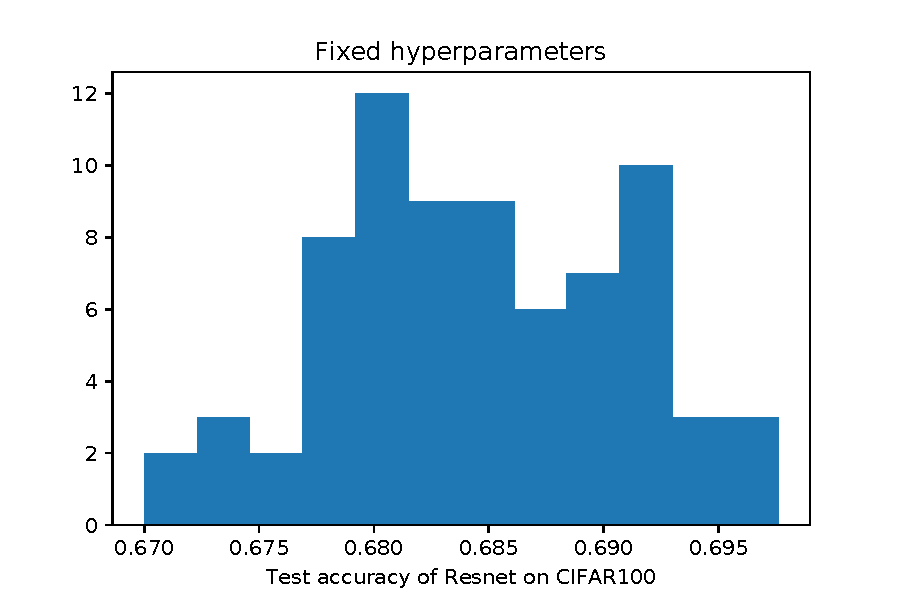
\includegraphics[width=\textwidth]{figures/resnet_hist.pdf} 
            \label{fig:resnet-hist}
            \caption[]{}
        \end{subfigure}
        \begin{subfigure}[b]{0.31\textwidth}
            \centering
             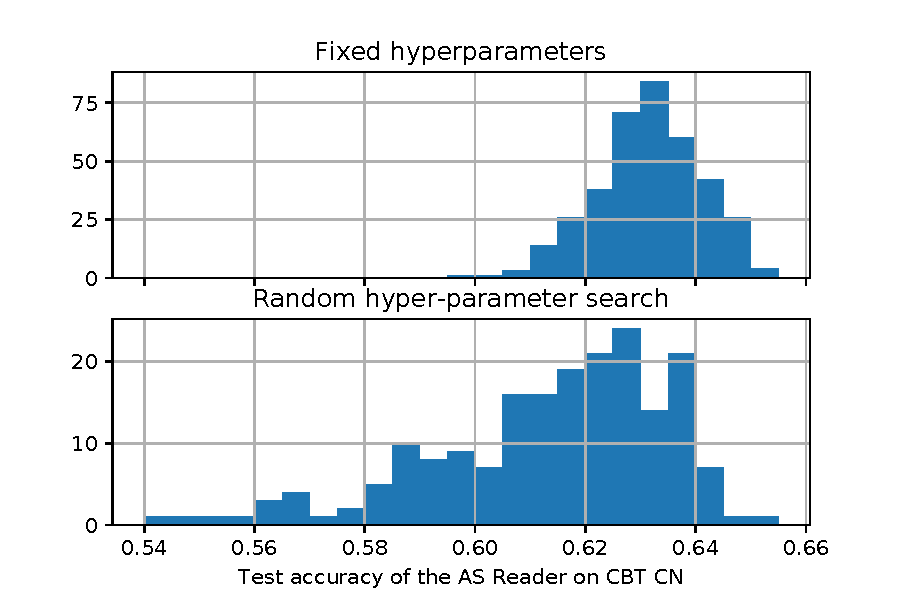
\includegraphics[width=\textwidth]{figures/asreader_cbt_cn.pdf}
            \label{fig:cbt-hist}
            \caption[]{}
        \end{subfigure}
%        \baselineskip
        \begin{subfigure}[b]{0.31\textwidth}   
            \centering 
            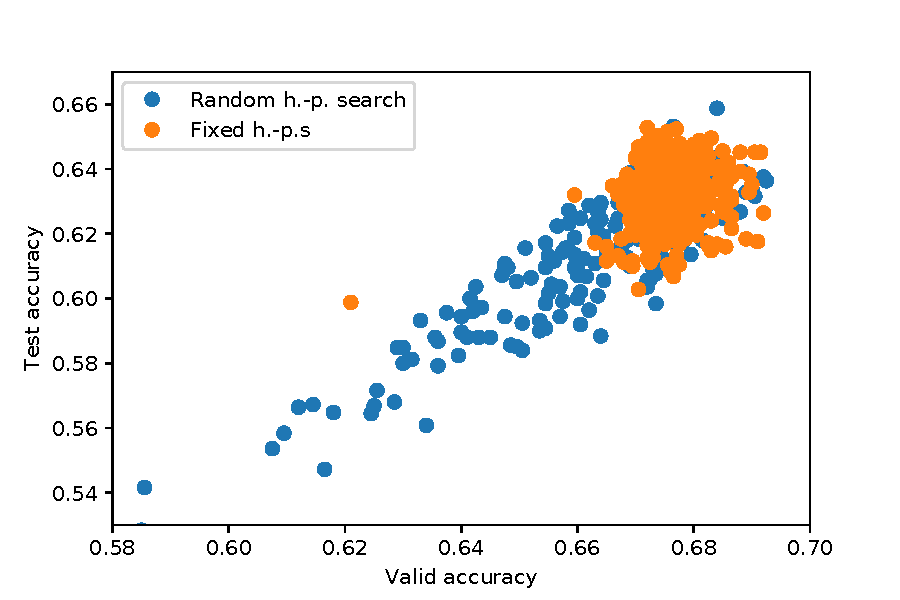
\includegraphics[width=\textwidth]{figures/cbt_valid_test.pdf}
            \label{fig:val-test-corr}
           \caption[]{}
        \end{subfigure}
        \caption[ NA ]{
        (a) \& (b) Distribution of test accuracies of 75 instances of Resnet evaluated on CIFAR100, 370 instances of the AS Reader model with fixed hyper-parameters and 197 with random hyperparameters trained and evaluated on CBT Common Noun subset. (b) Relationship between the test and validation accuracies of the AS Reader for random hyper-parameter search and for fixed hyper-parameters.}
        \label{fig:asr-test-accuracies}
\end{figure*}



\section{Experiment Results}
\label{sec:experiments}




{\it Note: The data and code for their analysis can be found at \url{http://gitlab.com/obajgar/boon}, along with Python functions you can use to calculate \tboon.}

We have run several experiments to quantify the scope of the problems outlined in Section~\ref{sec:intro-bestsinglemodel}. We just briefly summarize the main results here for illustration; a more detailed description of the experiments and analysis in the form of an iPython notebook can be found in the Gitlab repository.






\paragraph{Performance variation} To estimate the random variation of results, we repeatedly
\footnote{Specifically, 74 times for Resnet, 370 times for the AS Reader with fixed hyperparameters, and 197 times for the AS Reader with random hyperparameters.} 
trained models from two domains of \dl: the ResNet~\citep{he2016deep} on the CIFAR-100 dataset \citep{krizhevsky2009learning} to represent Image Recognition and the \asr \citep{Kadlec2016} on the \cbtcn \citep{hill2015goldilocks} to represent Reading Comprehension. Each of these trainings generated a pair of a validation and test performances.The resulting empirical performance distributions are illustrated in Figure~\ref{fig:asr-test-accuracies}. If we fix all hyper-parameters, the interquartile ranges of the models' accuracies are $0.98\%$ and $1.20\%$ (absolute). Compare this to the median differences between published results on these datasets: $0.86\%$ and $1.15\%$ respectively\footnote{We looked at results of successive architectures evaluated on the two tasks as listed in \cite{huang2016densely, munkhdalai2016reasoning}. We sorted the results with respect to the test performance and then calculated the differences between successive models. From these we calculated the median. Full details can be found in the Gitlab repository.}. Hence, random variation in performance cannot be considered negligible as is now often done.
Furthermore, if we allow the hyper-parameters to vary (in our case by random search), the result variance further increases, which further amplifies the outlined effects. In the case of the AS Reader the interquartile range increased to $2.9\%$ when we randomly picked hyper-parameters from a range applicable to training the model on a single GPU. However, note that the problem of result incomensurability due to hyper-parameter optimization is \emph{not} the focus of this work. The method that we present here is still applicable to the problem in the case of \emph{random} hyper-parameter sampling for which we include results, however we aim to compensate mainly for randomness due to parameter initialization and data shuffling -- which is however significant in itself, as we have just demonstrated. 

%For illustration Figure~\ref{fig:asr-test-accuracies} also shows the performance of he AS Reader when a random hyperparameter search is performed.

Several other articles confirm significant variation in model performance due to different random seeds: e.g van den Berg et al. \yrcite{Berg2016} in Speech Recognition, Henderson et al. \yrcite{henderson2017deep} in Deep Reinforcement Learning, or Reimers \& Gurevych \yrcite{reimers2017reporting} in Named Entity Recognition. They all agree that reporting performance scores of single models is insufficient to characterize architecture performance. 

\paragraph{Estimator variance} Figure~\ref{fig:conf-ints} shows the $95\%$ confidence intervals of best single model results compared to the $\boo{5}$ performance for a range of result-pool sizes $m$. This is shown for the cases of both strong and weak test-validation correlation. In both cases $\boo{5}$ is significantly less noisy than the best-single-model result. In fact in the case of random hyper-parameter search, \tboon shows even smaller variation than the mean (due to the negative skew of the performance distribution).

\begin{figure*} [t]
        \centering
        \begin{subfigure}[b]{0.475\textwidth}
            \centering
            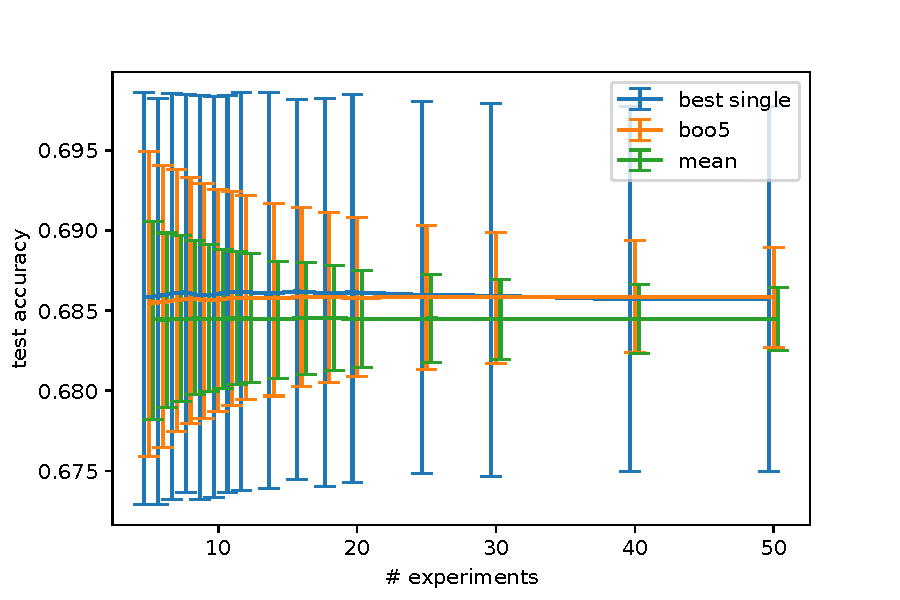
\includegraphics[width=\textwidth]{figures/resnet_conf_ints.pdf}
            \caption[]{Resnet~~ (fixed hyperparameters; low test-validation correlation)}    
            \label{fig:resnt-conf-ints}
        \end{subfigure}
        \hfill
%        \baselineskip
        \begin{subfigure}[b]{0.475\textwidth}   
            \centering 
            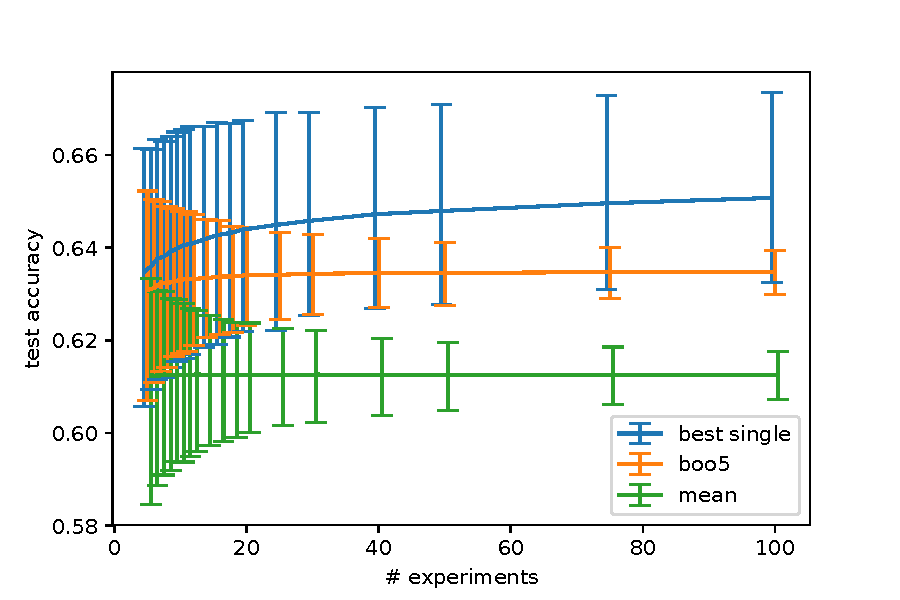
\includegraphics[width=\textwidth]{figures/cbtrs_conf_ints.pdf}
            \caption[NA]{AS Reader (random hyperparameter sampling; high test-validation correlation)}    
            \label{fig:asreader-conf-ints}
        \end{subfigure}
        \caption[ Averages and confidence intervals for the three ways of aggregating results. ]{Averages and 95\% confidence intervals of test performance for three ways of aggregating results of multiple experiments for various numbers of experiments run. Each confidence interval was constructed using smoothed\protect\footnotemark~Bootstrap sampling from our pool of 75 for Resnet and 197 experiments for the AS Reader with fixed and random hyperparameters respectively. Since we strongly encourage researchers to provide confidence intervals for their results, we provide and overview of how to construct them using the Bootstrap in Appendix~\ref{app:conf-ints}. }
        \label{fig:conf-ints}
\end{figure*}



\paragraph{Best-model performance improves with the number of experiments} We also mentioned that if only the performance of the best model is reported, the more experiments are run, the better the expected result. Figure~\ref{fig:asreader-conf-ints} illustrates that this effect can indeed be fairly strong, if the validation performance is a good predictor of the test performance, as is the case of the \asr with random hyper-parameter search, where the expectation of the best single model performance increases from $61.3\%$ if we train it once, to $63.3\%$ if we train it 5 times, to $63.5\%$ for 20 times. This effect is further explained e.g. by Jensen \& Cohen \yrcite{jensen2000multiple}. It gives a further argument for refraining from using this method and certainly also for publishing the number of experiments run, which is often not done. \tboon is not subject to this effect.

\paragraph{Validation-test correlation} However, note that the assumption that validation performance is a good predictor of test performance is sometimes not true. In the two cases with fixed hyper-parameters that we looked at, the Spearman correlation between validation and test results was only $0.10$ and $0.18$ respectively for the two models. The correlation significantly increases if we allow the hyper-parameters to vary -- to $0.83$ for the \asr. These results are also illustrated in Figure~\ref{fig:asr-test-accuracies}. Larger validation sets are also likely to improve this correlation, which can be understood as the degree of generalization from validation to test. 
Note that the problem of increasing expected performance mentioned above is relevant only in the case of higher correlation between validation and test results. The effect becomes very strong in the case where the performance we are reporting is also used for choosing the best model, which emphasizes the need for honest separation of validation and test data. 


\footnotetext{While \tboon and mean could be sampled using vanilla Bootstrap, best-validation result  is influenced only by a single value from the sample and hence uses only few values from the upper tier of our result pool, which makes our pool size insufficient. Hence we use Gaussian kernel smoothing~\citep{scott1992multivariate} to expand our result pool.}

% \subsection{Confidence intervals}

% Let us use the Bootstrap~\citep{Efron79} to estimate the confidence intervals for various sample sizes $m$ for the AS Reader\footnote{Usual Bootstrap draws samples from a pool of $m$ to estimate the variance of the estimator applied to a sample of size $m$. Here take advantage of our full pool of 370 observations to get a more precise estimate.}. We resampled samples of sizes $m=10, 25, 50, 100, 200$ from our pool of 370 observations $B=100,000$ times each. Each sample was used to calculate either the best-validation test result or $\boo{5}$.

% % The results are listed in Table~\ref{tab:confInts}, and they suggest, for instance, that we may need as many as 100 models to show that $\Em{5}$ accuracy of the AS Reader with the given fixed hyper-parameters is superior with at least $95\%$ confidence than $63.0\%$ -- the single model performance of the Memory Networks~\cite{hill2015goldilocks}, the previous model published for \cbtcn\footnote{However, the Memory Networks result is probably the best single model from an unknown pool, so this comparison is not entirely fair. This also points to the problem of transition to more robust statistical testing -- there is often not enough evidence in existing papers for robust statistical comparison. These may hence need to be re-implemented to then generate a sufficiently large sample from their performance distribution.}. However, importantly, the confidence interval is significantly narrower than the one for the best-single-model result. Since such a large amount of evidence is needed 
% \todo[inline]{Scrap comparison with MNs.}
% \todo[inline]{Replace table by a picture?}

% \begin{table*}
% \begin{center}
%   %\resizebox{\textwidth}{!}{
% %  \centering
%   \begin{tabular}[t]{l|rl|rl}%{@{}l@{~}r@{~~}r@{~~}r@{}l@{}r@{~~}r@{~~}r@{}l@{}r@{~~}r@{~~}r@{}l@{}r@{~~}r@{~~}r}
%     \toprule
%     {\bf Sample size $m$} & \multicolumn{2}{c|}{{\bf Best single}}  & \multicolumn{2}{c}{{\bf $\boo{5}}} \\

%     %\cmidrule{2-4} \cmidrule{6-8} \cmidrule{10-12} \cmidrule{14-16}
%     %& train & valid & test && train & valid & test && train & valid & test&& train & valid & test \\
%     \midrule
%     10 &[61.6 & 64.6] & [ 62.4 & 64.1 ]\\
%     25 &[61.7 & 64.5] & [ 62.7 & 63.9 ]\\
%     50 & [61.8 & 64.5] &[ 63.0 & 63.7 ]\\
%     100 &[61.8 & 64.5] &[ 63.1 & 63.6 ]\\
%     200 &[61.8 & 64.5]\todo{use Gaussian interpolation to get finer estimates} &[ 63.2 & 63.5 ]\\

%     \bottomrule
%   \end{tabular}
%   %}
% \end{center}  
  
%   \caption{$95\%$ confidence intervals of $\emn$ of the \asr for various sample sizes. Each of these was constructed using $B=100,000$ Bootstrap samples.}
%     \label{tab:confInts}
% \end{table*}


\section{Discussion}
\tboon does fix the main flaws of reporting the best single model performance. However, let us have a look at some of its limitations.

\paragraph{Hyperparameter tuning} This work does not fully compensate for improved expected results due to hyperparameter tuning, nor was it its primary aim. \tboon is appropriate in the case of random hyperparameter sampling, where the performances in different runs are independent. However, this is not the case for more advanced hyperparameter optimization methods. The primary focus of this work was on tackling variability due to random initialization, data shuffling, and similar sources, which we have shown to be significant in itself. Compensation for more advanced hyperparameter tuning (and ensuring the comparability of models in that case) is certainly a worthwhile area for future research. 

\paragraph{Mean, median, and other alternatives} We do not claim our method to be strictly superior to traditional ways of aggregating results, such as mean or quantiles. However, we have outlined a case where using \tboon is justified -- situations where a final model to be deployed can be chosen from a pool of trained candidates. In such case, \tboon is easily interpretable and more informative than a performance of a typical model, expressed by mean or median. Hence, we think \tboon is a useful addition to the methodological toolbox along existing methods.


\paragraph{Just a single number} \tboon is still just a single number whose ability to characterize the performance distribution is limited by its single dimension. Paper authors should try to characterise the performance distribution as fully as possible, which may involve a histogram, mean, standard deviation, ideally along a dataset containing the results of all experiments, from which an interested reader may be able to deduce whichever characteristic she finds interesting. Unfortunately, such characterization is usually lacking.

However, \emph{alongside} this detailed characterization, describing an architecture's performance by a single number still has its appeal, especially for the purpose of comparison among architectures and choosing the best one according to some criterion (in fact, each quantitative score can be understood as a proxy for ordering architectures with respect to such criterion of interest, such as expected performance of the best model out of $n$). We have explained why, in some cases, \tboon may be useful for such purpose. 

\paragraph{Computational cost} Some may deem \tboon impractical due to its requirement to train architectures many times, which may be very expensive in some cases. However, result stochasticity needs to be addressed to produce reliable results, and it is hard to imagine a general method to do so without repeated evaluation\footnote{Though different methods can substantially differ in the number of evaluations that they require.}. Researchers can simply focus on architectures which they can evaluate properly given their resources. However, the main target of our criticism is not projects whose resources are stretched by a single training; it is projects that do have the necessary resources for multiple evaluations but use them to produce better-looking results rather than results that are more informative and robust.


\section{Conclusion}
Reporting just the best single model performance is not statistically sound. This practice in machine learning research needs to change if the research is to have lasting value. Reviewers can play an important role in bringing this change.

Still, asking for the performance of a best model out of $n$ can have valid reasons. For the situations where the best-model performance is indeed a good metric, we are suggesting \tboon as a way to evaluate it properly. 

\vskip 0.1in



\begin{appendices}


\section*{Appendix}
\section{\tboon of the Gaussian Distribution}
\label{app:gaussian}

In this section we will calculate \tboon of the Gaussian distribution. This can serve as a basis for a parametric estimator of \tboon, when we assume a performance distribution to be (approximately) Gaussian, which was the case of some of the performance distributions we have examined, for instance the AS Reader with fixed hyper-parameters.

\subsection{Single evaluation dataset}

In the simpler case in which the best model is chosen with respect to the same dataset on which the performance is then reported, we can substitute the \pdf and \cdf of the Gaussian distribution into Equation~\ref{eq:expMax} to get
\begin{multline}
\overline\emn(\mathcal{N}(\mu,\sigma^2)) = \\ \int_{-\infty}^\infty x n \frac{1}{\sqrt{2\pi\sigma^2}}e^\frac{(x-\mu)^2}{2\sigma^2} \Phi^{n-1}\left(\frac{x-\mu}{\sigma}\right) dx
\end{multline}
where $\Phi$ is the \cdf of a standard normal random variable. Substituting $z=\frac{x-\mu}{\sigma}$, $dx=\sigma dz$, yields
\begin{multline}
 \int_{-\infty}^\infty  n (\mu+\sigma z)  \frac{1}{\sqrt{2\pi\sigma^2}}e^\frac{z^2}{2} \Phi^{n-1}\left(z\right)\sigma dz = \\
$$ = \mu \int_{-\infty}^\infty  n  \frac{1}{\sqrt{2\pi}}e^\frac{z^2}{2} \Phi^{n-1}\left(z\right)dz + \\
+\sigma\int_{-\infty}^\infty  n  z  \frac{1}{\sqrt{2\pi}}e^\frac{z^2}{2} \Phi^{n-1}\left(z\right) dz = \mu + \sigma\overline\emn\left(\mathcal{N}(0,1)\right)
\end{multline}
(the first integrand has the form of the \pdf found above and hence integrates to one) so the expected maximum is neatly expressed in terms of a maximum of a standard normal and is linearly proportional to both the mean and the standard deviation. Once $n$ is fixed for comparison purposes, $\emn\left(\mathcal{N}(0,1)\right)$ is just a constant, e.g. $\Em{5}\left(\mathcal{N}(0,1)\right)\approx1.163,\;\Em{10}\left(\mathcal{N}(0,1)\right)\approx1.539$.

\subsection{Test-validation evaluation}
\label{app:gaussianTV}
Let us turn to the case of reporting a test set performance of a best-validation model. If we model the validation and test performances by a Bivariate Normal Distribution with valid-test correlation $\rho$, means $\mu_\text{val},\mu_\text{test}$, and variances $\sigma_\text{val}^2, \sigma_\text{test}^2$, then given a validation performance $\xval$, the test performance is distributed normally with conditional expectation
$$E_{tv}(\xval) = \mu_\text{test} + \rho \frac{\sigma_\text{test}}{\sigma_\text{val}} \;(\xval - \mu_\text{val})$$
which gives
\begin{multline}
\emn(\mathcal{N}(\mu,\sigma^2)) =  \\
\int_{-\infty}^\infty  \left(\mu_\text{test} + \rho \; \frac{\sigma_\text{test}}{\sigma_\text{val}} (\xval - \mu_\text{val}) \right) n \cdot \\ \cdot \frac{1}{\sqrt{2\pi\sigma_\text{val}^2}}e^\frac{(x-\mu_\text{val})^2}{2\sigma_\text{val}^2} \Phi^{n-1}\left(\frac{x-\mu_\text{val}}{\sigma_\text{val}}\right) dx \;. 
\end{multline}

Using the same two tricks as above, this can be simplified to
\begin{multline}
\label{eq:gaussExpMax2}
 \emn(\mathcal{N}(\mu,\sigma^2)) = \mu_\text{test}+ \rho\;\sigma_\text{test}\;\overline\emn\left(\mathcal{N}(0,1)\right) 
\end{multline}
where $\overline\emn\left(\mathcal{N}(0,1)\right) $ is the single-evaluation expected maximum of the standard normal distribution as defined above. 


\bibliographystyle{icml2018}
\bibliography{references}


% \section*{Other Appendices}
% \hypertarget{app:metastudy-details}{}
% \hypertarget{app:conf-ints}{}


% {\it The article with all appendices can be found as a supplement to the ICML submission, in the Gitlab repository (\url{https://gitlab.com/obajgar/boon}), or on arXiv.}
% \end{appendices}


\section{Survey of ICLR 2017 Papers: Method}
\label{app:metastudy-details}

We downloaded the pdfs of all papers accepted to ICLR 2017\footnote{Downloaded from https://openreview.net/group?id=ICLR.cc/ /2017/conference from sections "Paper decision: Accept (Oral)" and "Paper decision: Accept (Poster)".}, extracted text from them using the OpenSource Xpdf package\footnote{http://www.xpdfreader.com/; we used version 4.00.01 on Debian Linux 9.2.} and then searched the resulting text documents using the grep command as follows. %\todo[inline]{Provide code?}

Firstly, to roughly estimate the usage of experiments in the papers, we searched for the capitalized string "EXPERIMENT" in the documents, since all (sub-)section headings are capitalized in the ICLR format. This was matched in 174 documents. Further 6 contained the string "EVALUATION" yielding a total of 180 out of 194 papers containing one of the two strings, which suggests that many ICLR papers indeed have an empirical component, though our rough method is only very approximate.

We then searched for the string "confidence interval", which was matched in only 11 papers, and further 11 documents matched one of expressions related to hypothesis testing (curiously, a set completely disjoint from the "confidence interval" set). These terms were: "hypothesis test", "p-value", "t-test" "confidence level", "significance level", "ANOVA", "analysis of variance", "Wilcoxon", and "sign test". This may actually be only an upper bound since mentioning the term somewhere in the paper does not necessarily mean that the method was employed in the experimental procedure.



\section{Experiments: Details}
\label{app:experiments}

{\it Note: The data and code for their analysis will be available at \url{http://gitlab.com/obajgar/boon}.}

Here we provide further details of our experiments quantifying the extent of result stochasticity and the resulting effects. 

\subsection{Models}

To run our experiments we have chosen Open Source implementations\footnote{The source code for Resnet can be found at \url{https://github.com/tensorflow/models/tree/master/research/resnet}; the code for the \asr at \url{https://github.com/rkadlec/asreader}.} of models from two popular domains of deep learning, namely ResNet~\citep{he2016deep} on the CIFAR-100 dataset \citep{krizhevsky2009learning} for Image Classification and the \asr \citep{Kadlec2016} on the \cbtcn dataset \citep{hill2015goldilocks} for Reading Comprehension. We believe these two models are representative of models in their respective areas -- Resnet is based on a deep convolutional network architecture as most recent models in machine vision, while the AS Reader is based on a bidirectional GRU network with attention, as is the case for many models in Natural Language Processing. 


\subsection{Data collection}
To collect the data for our experiments, we repeatedly trained the two models. Each training instance had a different random parameter initialization and random data shuffling. We evaluated the model on the validation and test datasets at least once per epoch. We then took the validation and test performance at the best-validation epoch as a data point for our further analyses.

All training was done on Ubuntu 14.04 on a single GPU per training, either Nvidia Tesla K80 or GTX 1080.

\subsubsection{Resnet}
Resnet was trained with a single set of hyperparameters, the default ones for the above Open Source implementation. That means 5 residual units resulting in a 32-layer Resnet. The model was trained using the 0.9 momentum optimizer, with batch size 128, initial learning rate of 0.1 lowered to 0.01 after 40,000 steps and to 0.001 after 60,000 steps. Data augmentation included padding to 36x36 and then random cropping, horizontal flipping and per-image whitening. L2 regularization weight was set 0.002. 

Training was done using Tensorflow 1.3.

\subsection{AS Reader}
The AS Reader was trained in two different settings. Firstly 370 times with hyper-parameters fixed to embedding dimension of 128 and 384 hidden dimensions in the GRU units, with all other hyper-parameters as used in the original AS Reader paper \citep{Kadlec2016}.

In the second setting, the hyper-parameters for each training instance were chosen randomly from the following ranges: The batch size was chosen from the range $[16,128]$, and the embedding size and hidden state size were each chosen from the range $[16,512]$ with the $\log_2$ value of the parameter being distributed uniformly in the interval. Parameters from these ranges worked reasonably well in our preliminary experiments.

Training was done using Theano 0.9.0 and Blocks 0.2.0.

\subsection{Performance distribution results}
\label{sec:perfDists}

% % We will now demonstrate that model performance is indeed stochastic for multiple successful models from several areas of \ml, namely text comprehension, image classification, and knowledge base completion. The fact that model performance is stochastic due to random parameter initialization and data shuffling is well known and has been pointed out for instance by~\cite{Berg2016, bisani2004bootstrap, henderson2017deep,reimers2017reporting}, however it is almost never mentioned in articles proposing new models, so we believe it useful to demonstrate it in the context of this article. 

% For our experiments, we chose models which achieved competitive performance in their respective fields on some frequently used evaluation task, are in some sense typical of the structure of models used in that field, and have a reasonable training time, so that we could run a sufficient number of experiments to estimate their performance distributions. In particular we chose the following models and tasks: ResNet~\cite{huang2016densely} on the CIFAR-100 dataset \cite{krizhevsky2009learning} for image classification; the \asr \cite{Kadlec2016} on the \cbtcn dataset \cite{hill2015goldilocks} for Reading Comprehension; and the DistMult model \cite{Yang2015} on the FB15k dataset \cite{Bordes2013} as used in \cite{kadlec2017knowledge} for Knowledge Base Completion. In our results, we also include results of experiments from \cite{Berg2016} on Speech Recognition. 




% \begin{table*}
% \begin{center}
%   %\resizebox{\textwidth}{!}{
% %  \centering
%   \begin{tabular}[t]{lrr|rr|rr|r|r}%{@{}l@{~}r@{~~}r@{~~}r@{}l@{}r@{~~}r@{~~}r@{}l@{}r@{~~}r@{~~}r@{}l@{}r@{~~}r@{~~}r}
%     \toprule
%     {\bf Model} & {\bf Dataset} & {\bf Metric} &  \multicolumn{2}{c|}{\bf 95\% conf. int.} & {\bf Mean} & {\bf SD} & {\bf median $\delta$} & {\bf t.-v. corr.}\\

%     %\cmidrule{2-4} \cmidrule{6-8} \cmidrule{10-12} \cmidrule{14-16}
%     %& train & valid & test && train & valid & test && train & valid & test&& train & valid & test \\
%     \midrule
%     AS Reader~\cite{Kadlec2016}   & \cbtcn   & Error  & 35.24   & 38.87 & 36.84 & 0.94& 1.15 & 0.18\\
%     %DistMult~\cite{Yang2015,kadlec2017knowledge} & FB15k & Hits@10  & 84.92   & 85.26   & 85.15  0.15 &  1.40   & 0.38\\
%  %   DenseNet~\cite{huang2016densely}  & CIFAR-10  & Error  &  5.39     & 6.01   & 5.70 & 0.16 & - & N/A \\
%     ResNet~\cite{he2016deep} & CIFAR-100 & Error & 26.54 & 37.76 & 31.54 & 0.62 &0.86& 0.14\\
% %    DNN/CNN~\cite{Berg2016}\footnote{Results taken from \cite{Berg2016} and were averaged over the 5 experiments varying both data shuffling and initial parameters - i.e. for two architectures (DNN and CNN) and 4 datasets (BN50, BN400, SWD Hub5, SWD-CallHome).} \todo{ask for full data} & BN & N/A & N/A & 17.11 & 0.20 & ? & NA \\ 
%     \hline
%     AS Reader (HPS )& \cbtcn & Error     &  35.99   & 43.49  & 36.83  & 2.48  & 1.15 & 0.84 \\
%  %   DistMult (HPS)  & FB15k & Hits@10  & 45.45   & 89.02    & 80.25  & 20.92&1.40   & 0.97\\

%     \bottomrule
%   \end{tabular}
%   %}
% \end{center}  
  
%   \caption{Characteristics of performance distributions of several \ml models. `t.-v. corr.' is the Spearman correlation between the validation and test results. (HPS) marks models for which we performed a random hyper-parameter search while constructing the sample. }
%     \label{tab:perf-dists}
% \end{table*}


Figure~\ref{fig:asr-test-accuracies} plots the histograms of test performances of the evaluated models. The mean test accuracy for Resnet was $68.41\%$ with standard deviation of $0.67\%$ (absolute), the range was $67.31\% - 69.41\%$. For AS reader with fixed hyperparameters the mean was $63.16\%$ with standard deviation $0.94\%$ and range of $61.52\% - 64.60\%$.   In the case of random hyper-parameter search the mean was $61.26\%$, standard deviation $2.48\%$, and values ranged from $56.61\%$ to $64.01\%$.

In both cases with fixed hyper-parameters the collected results are consistent with coming from a Gaussian distribution according to the Anderson-Darling test\footnote{That is, despite the relatively large sample sizes, gaussianity cannot be ruled out at $0.05$ significance level based on collected evidence.}~\cite{anderson1954atest}; the histograms also make it appear plausible that the performance distribution is approximately Gaussian. This is not the case for the random hyper-parameter search where the distribution has a clear negative skew. 


To put the above numbers into context, we also examined the margin of improvement of successive architectures published on the corresponding datasets, as listed in \cite{munkhdalai2016reasoning, huang2016densely}. We sorted the results with respect to the test performance and then calculated the differences between successive models. The median difference was for $0.86\%$ for CIFAR-100 and $1.15\%$ for \cbtcn. 
% For the \asr and DistMult we also list results for a sample constructed while conducting hyper-parameter search. In the case of the \asr we chose the hyper-parameters randomly from an interval of values that gave reasonable results in preliminary experiments\footnote{Specifically, we chose batch size from the range $[16,128]$, and the embedding and hidden state dimensions from the range $[16,512]$ using the reciprocal distribution in all three cases.}; in the case of DistMult, the parameters were chosen by hand knowing the results of previous experiments. These are two of possible modes in which hyper-parameter search can be conducted. We include these results to reflect the fact that in practice, when models are trained repeatedly, it is usually with different hyper-parameters, although re-running experiments with fixed hyper-parameters is also something worth encouraging.

Note that the median differences are smaller than two standard deviations for each model. Two standard deviations from the mean approximately give the $95\%$ confidence interval for a Gaussian distribution -- hence we could typically fit three successive published results within the width of one such confidence interval. The magnitude of the performance variation due to random initialization and data shuffling is therefore not negligible compared to the improvements in performance, which often hold an important place within articles in which they are presented. We hence think it is inappropriate to completely ignore this random variation in evaluation protocols, which is currently the usual practice. 


\subsection{Test-validation correlation}
\label{sec:tv_corr}

The best model is usually selected using validation performance
\footnote{Or at least should be.}.
This practice is based on the assumption that the validation accuracy is a reasonably good predictor of test accuracy. The results of our experiments, illustrated also in Figure~\ref{fig:asr-test-accuracies}, suggest that this assumption holds for performance variation due to hyper-parameter choice. However, if we fix the hyper-parameters, the correlation almost disappears. To some extent, this implies that selecting the best validation model means we are picking randomly with respect to the test performance. Since we are picking from a random test performance distribution, this further calls for better characterization of the distribution than a single instance drawn from it. 

On the other hand if the correlation is strong, as seems to be the case if we do perform hyper-parameter search, we face the second problem with reporting the best-validation performance:



\subsection{Effect of the number of experiments}



If the validation performance is a good predictor of the test performance, then the more models we train the better the best-validation model is likely to be even on the test set since we are able to select models high up the right tail of the performance distribution. This effect has been described in more detail in~\cite{jensen2000multiple}, though with focus on induction algorithms; here we present an estimate of its effect in the case of Resnet and \asr.

To test this effect we took the pool of trained models. For each $m$ in the range from $1$ to $50$ (or $100$ for the \asr), we randomly sampled $100,000$ samples of size $m$ from the pool, and selected the best-validation model from each sample. The mean test performance across the $100,000$ samples for each $m$ is plotted in Figure~\ref{fig:conf-ints}. %We also include the case where the best model is picked directly with respect to its test performance, mainly to re-emphasize why such practice should be avoided.


The results show that when there is suitable correlation between validation and test performances, increasing the number of experiments does increase the expected performance of the best-validation model. This makes the number of experiments an important explanatory variable, which however usually goes unreported. Furthermore, it makes results reported by different research teams not directly comparable. Finally, it gives an advantage to those that can run more experiments. We believe that this again makes the practice of reporting the performance of the best single model unsuitable. 



% \section{Formal description of performance stochasticity}
% \todo{Candidate for removal}

% This work is based around the idea that any measured performance of a \ml{} model can be understood as a random variable drawn from some probability distribution $\mathfrak{P}$ which we shall call the \emph{performance distribution}. Let us now explain in more detail how this stochasticity arises. 

% Assume we are trying to solve a problem using machine learning. Then we are trying to find a function (a model) that would correctly map an input (e.g. an image, or a text document and a question) from set $X$ to an output (e.g. image class or an answer to that question) from a set $Y$. Then by a \emph{model architecture} we will mean a class $M$ of functions $M_{h_M,W}:X\to Y$ where $h_M$ is a tuple of model hyperparemeters (e.g. number of hidden dimensions, number of layers) and $W$ is a tuple of trainable parameters of the model. 

% Let $X^\text{train}=\left(x_1^\text{train}, \dots, x_{N^\text{train}}^\text{train}\right)\in X^{N^\text{train}}$ be the training set. Then a training algorithm generally takes in a training sequence $\mathbf{x}^\text{train}=(x_{i_1},x_{i_2},\dots,x_{i_T})$ and initial values of parameters $W_0$ and returns new values of $W_T$ of the trained parameters, which are in some sense optimal with respect to the training data. 

% These are the two points where stochasticity usually comes into play. The training sequence is usually created by concatenating different uniform random permutations of the training set - we usually call the number of these different permuations the number of epochs. The initial parameter values are then drawn from some initialization distribution - often uniform or normal, but special initialization methods are used for some network components, such as random orthogonal matrices~\cite{Saxe2014}.

% The training algorithm (with hyper-parameters $h_\tau$) can then be understood as a (deterministic) function $\tau_{h_\tau}$, which takes in the model $M_{h_M}$\todo{nove znaceni}, its initial parameter values $W_0$, and the training sequence and produces the final parameter values $W$. The final measured performance of the model is then a function of the model, the final parameters and some test set\todo{The test set can be understood as part of this function, which can then be understood as any testing procedure}. By composing this performance function with the training function, the model performance is a deterministic function of pre-set arguments $h=(h_M, h_\tau)$ and random arguments $\mathbf{x}^\text{train}$, $W_0$. Deterministic function of random variables generally produces another random variable. Hence the training and evaluating a model can be in this sense understood as drawing a random variable $P$ (the model performance) from a random distribution $\mathfrak{P}_h$. This performance distribution is what characterizes performance of a single model architecture. \todo{expand}


\begin{figure*} [ht]
        \centering
            \centering
            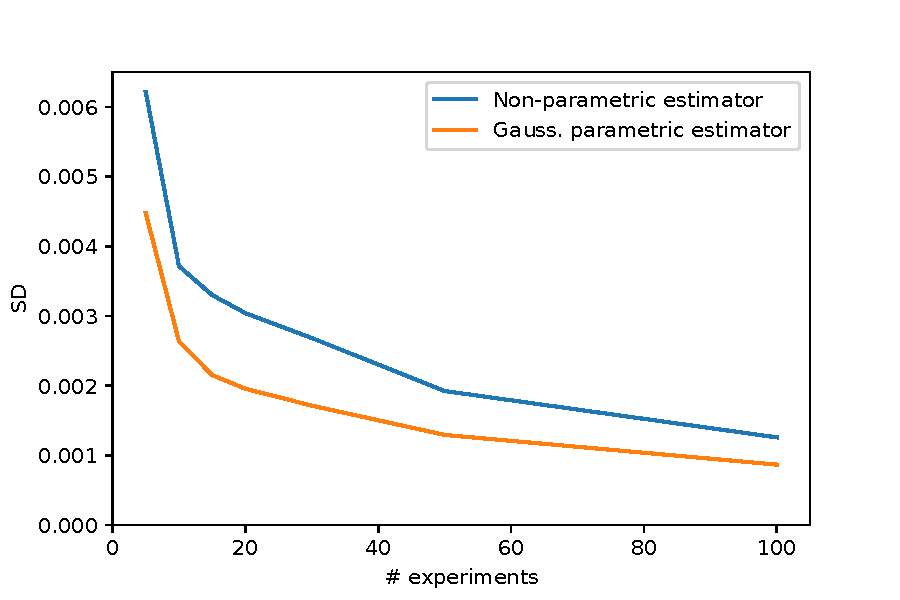
\includegraphics[width=0.6\textwidth]{figures/param_non_param_comparison.pdf}
        \caption[ NA ]{
        Empirical comparison of the variances of the non-parametric and Gaussian parametric \tboon estimators. The data come from experiments with the AS Reader on CBT with fixed hyperparameters.}
        \label{fig:estimator_comparison}
\end{figure*}


\section{Dealing with Estimator Uncertainty}

\subsection{Confidence intervals}
\label{}
If an estimator characterizing a performance distribution, say  $\widehat{\emn}$ or average, is calculated from experimental observations, it is subject to random variation, so if another research team tries to reproduce the experiments, they generally get a different estimate. The more observations are collected, the more precise the estimate generally is. Confidence intervals provide a natural way to express this uncertainty. Their usage also gives a sense whether the number of performed experiments was sufficient to reduce the uncertainly to a reasonable level, which is again not frequently addressed in \ml papers. 

The construction of the confidence interval would be trivial if we knew the distribution from which our estimate was drawn (as opposed to the distribution of the performance!) -- it is simply the interval between the appropriate quantiles, e.g. the 2.5th and 97.5th quantiles in the case of the $95\%$ confidence interval. Such distribution has been studied extensively for instance in the case of a mean of Gaussian random variables. However, in other cases, it is not known. If we know at least the distribution from which the individual observations were drawn, we can use Monte Carlo methods to precisely estimate the confidence interval; however, if we are not able to make an assumption about the underlying distribution, we need to use only what we have: our samples from the distribution. In such case the variability of our estimator can be approximated using the Bootstrap~\citep{efron79} or similar methods. 

The Bootstrap consists of repeatedly sampling \emph{with replacement} $m$ random observations from our pool of $m$ observations, say $B$ times. Each such sample is then used to calculate an estimate of our quantity of interest, say $\emn$ or mean. This creates a sample of $B$ values of the estimator. The confidence interval can then be easily estimated taking the appropriate quantiles from this resulting \emph{Bootstrap} distribution of the estimator, which should be approximating the unknown underlying sampling distribution. The Bootstrap distribution has been shown to converge to the true underlying performance distribution.

If we know the underlying distribution (up to some parameters), we can estimate its parameters and then generate a simulated \emph{Monte Carlo} sample from the distribution, which can be used to calculate a sample of the estimator and the corresponding confidence interval in a similar way as above with the advantage of the distribution being smoother.


Beside estimating the confidence interval for the value of $\emn$ or mean itself, either re-sampling method can be used to construct a confidence interval for the relative improvement of the newly proposed architecture compared to a baseline. The improvement can then be considered significant if zero is not included in the confidence interval. More details on constructing Bootstrap confidence intervals can be found in many standard texts on computational statistics, for instance in \cite{efron1987better}.

For illustration, we calculated the Bootstrap confidence interval for several sample sizes $m$ for Resnet and the AS Reader. Each was constructed using $B=100,000$. The results are plotted in Figure~\ref{fig:conf-ints}.%, and they suggest that we may need as many as 100 models to show that $\Em{5}$ accuracy of the AS Reader with the given fixed hyper-parameters is superior with at least $95\%$ confidence than $63.0\%$ -- the single model performance of the Memory Networks~\cite{hill2015goldilocks}, the previous model published for \cbtcn. 







% \subsection{Significance tests}

% \label{app:sigTests}
% An important point in many papers proposing new \ml{} architectures is a claim that the proposed model performs better than some baseline on some benchmark task\footnote{Whether so much focus should be put such benchmarking may be questionable; for a discussion of this topic see \cite{Church2017}.}. This amounts to saying that a certain metric $\theta_M$ characterising the proposed model $M$ is higher than that statistic $\theta_B$ of some baseline $B$. In our case the $\theta$ will be the expected maximal performance; in traditional hypothesis testing (e.g. in the $t$-test) it is often the population mean. 

% The test then amounts to showing that we should favour an alternative hypothesis
% $$H_1:\;\;\theta_M\geq\theta_B\;\;$$
% claiming that $\theta$ is higher for our model than for the baseline\footnote{Higher for quantities such as classification accuracy or BLEU score; the case where lower is better (e.g. cross-entropy, mean square error (MSE) or mean rank) can be handled in an analoguous way, examining the lower tail as opposed to the higher tail in what follows.} over a null hypothesis
% $$H_0:\;\; \theta_M = \theta_B.$$

% The statistic $\theta$ is a characteristic of the performance distributions $\mathfrak{P}_M$, $\mathfrak{P}_B$ of the proposed model and the baseline respectively -- how to compute the expected maximum from the underlying distribution was illustrated above. However we often do not have access directly to the underlying distribution, only a sample drawn from that distribution which allows us to compute an estimate $\hat{\theta}$ of $\theta$. 

% Since both estimates $\hat\theta_M$, $\hat\theta_B$ are noisy, if they are close to each other, simply stating that $\hat\theta_M \geq \hat\theta_B$ is not sufficient for showing that $\theta_M \geq \theta_B$ and therefore that the proposed model is (in some sense) better than the baseline. The difference in the estimates may be simply due to random noise. The hypothesis test calculates the probability that the stated difference in the empirical estimates occured due to random variation as opposed to a true difference in models' characteristics. 

% To do this, we calculate the probability that a difference in the empirical estimates of the parameters at least as extreme as the observed one occurs. If we know the sampling distribution from which the empirical estimates $\hat\theta$ come (which often stems from knowing the theoretical distributions $\mathfrak{P}$, at least up to a few parameter values) we can calculate this $p$-value exactly as is the case of the well-known $t$-test \cite{Student1908} for comparing means. However in many cases the underlying distribution is not consistent with the Gaussian assumption and such analytical methods may no be known for. Similarly such a method may not exist for statistics other than the mean. 

% In such a case a common way of estimating the $p$-value are methods based around the Bootstrap \cite{efron79}. Such a method allows us to estimate how variable our estimate of the metric $\theta$ is, i.e. how inaccurate our estimate possibly is. A more complete guide to hypothesis testing using Bootstrap methods can be found in \cite{Chernick07} or \cite{Mackinnon09}. 

% (...)\todo{General introduction into how Bootsrapping works}

% In the case of expected maximum we have our sample of $m$ performances of individual model instances $x_1, \dots, x_m$ which we can sort in descending order as $x_{i_1}\geq x_{i_2}\geq \dots \geq x_{i_m}$ and we can give an estimate of the Expected maximum as
% \begin{equation}
% \hat{\emn}=\frac{\sum_{j=1}^{m-n+1} {{m-j}\choose{n-1}}x_{i_j}}{{{m}\choose{n}}}
% \end{equation}
% \todo{Tenhle vzorec odvodit a vysvětlit v sekci o Expected max}
% where $ {m}\choose{n}$ is the binomial coefficient. 

% Bootstrapping consists of resampling samples of size $m$ with replacement from the empirical distribution which places probability mass of $\frac{1}{m}$ on each $x_i$. This is repeated $b$ times yielding samples $\{x_{1,1}, \dots, x_{1,m}\},\dots,\{x_{b,1},\dots,x_{b,m}\}$ from which we can calculate $b$ estimates $\hat\theta^*_1,\;\dots\;,\hat\theta^*_b$ of $\theta$.

% Now in traditional hypothesis testing we would test whether the statistic $|\hat\theta-\theta_B|$ is extreme enough to justify rejecting the null hypothesis $H_0$. This may lead us to think that $|\hat\theta^*_k-\theta_B|$ is the right Bootstrap of the test statistic. However the $p$-value calculation assumes that the empirical estimate is sampled under the null hypothesis $H_0$ - this is not the case for $\theta^*_k$. Hence as \cite{Hall91} point out, in Bootsrap hypothesis testing we should rather use the samples $|\hat\theta^*_k-\hat\theta|$ for determining the distribution of our test statistic $|\hat\theta-\theta_B|$. The second important point they also emphasize is that \todo{Check details of the second guideline (pivoting) in Beran 1987, 1988; test whether it is needed in our case.}

% To test for confidence level $(1-\alpha)$ (the most common choice being $\alpha=0.05$) we then need to find a critical value $\hat t$ for the test statistic $|\hat\theta-\theta_B|$ such that
% $$ \prob^*\left[\hat\theta^*-\hat\theta>\hat{t}\right] = \alpha$$
% where $\prob^*$ denotes the probability under the Bootstrap-based empirical distribution, i.e.
% $$ \prob^*\left[\hat\theta^*-\hat\theta>\hat{t}\right]  := \frac{\left|\left\{k \text{ such that }  \hat\theta^*_k - \hat\theta  > \hat{t}\right\}\right|}{b}$$
% (here the outer $|$ denotes set cardinality while the inner ones denote usual absolute value.).

% We then reject the hypothesis with confidence $(1-\alpha)$ if the statistic $|\hat\theta^-\theta_B|$ exceeds the critical value $\hat{t}$. 

% \subsection{Two-sample test}
% While the above testing procedure is suitable for situations where we want to compare a newly proposed model to a baseline for which we have only a single result available\footnote{Which is either normalized to a known number of experiment runs, or at least the number of times the experiments that have given rise to the result is known.}, sometimes we may have samples available from the performance distributions of both the newly proposed model and the baseline. This may be thanks to a public competition run via a platform like OpenML\footnote{http://openml.org}\cite{vanrijn13} which makes the results of individual runs available (in such a case statistical testing may be done directly by such platform); the results may be otherwise published by the authors of the baseline architecture, or we may have an implementation of the baseline architecture directly available and hence be able to generate the samples ourselves\footnote{Which may be the ideal experimental scenario since we can then suit the baseline experimental configuration precisely to the needs of our evaluation methodology and can ensure equal conditions to the baseline and the new model for example in what concerns hyper-parameter tuning.}. 

% In such a case we are testing the same hypotheses however this time $\theta_B$ is not a known single value -- as for the new model's performance distribution we only have access to samples from the underlying performance distribution. Our test statistic is now $|\hat\theta_M-\hat\theta_B|$ and the critical value $\hat{t}$ can now be found as a value satisfying
% $$ \prob^*\left[\hat\theta_M^*-\hat\theta_B^*>\hat{t}\right]  = \frac{\left|\left\{k \text{ such that }\;  \left(\hat\theta^*_{M,k} - \hat\theta_M + \hat\theta_B\right) - \hat\theta_{B,k}^*  > \hat{t}\right\}\right|}{b}<\alpha.$$
% Importantly note that we are shifting the Bootstrap distribution of the new model so that its expected maximum matches the expected maximum of the baseline since this is a central assumption of the null hypothesis and the Bootstrap samples should done under the null hypothesis.



% The null hypothesis (of no significant difference in model performance) is then rejected if $|\hat\theta_M-\ha





\section{Comparison of estimators}




Figure~\ref{fig:estimator_comparison} shows the comparison of the non-parametric and Gaussian parametric estimators of \tboon, both introduced in Section~\ref{sec:emp-estimation}, in terms of their variance for various sample sizes. The parametric estimator shows a somewhat lower variance. This is an advantage if the performance distribution is indeed approximately Gaussian, which is the case for both cases with fixed hyperparameters that we tested in our experiments. However, this can introduce bias if the true performance distribution differs from the theoretical distribution assumed by a parametric estimator, so one should be prudent to use it.

\end{appendices}










%#############              JUNKYARD               #######################

% \section{Case studies}
% Let us now demonstrate how to apply these tests in two situations that could arise in Reading Comprehension research. 
% \subsection{Single-sided test}
% First consider a situation where an earlier paper has introduced a model with test accuracy of $63.0\%$ on the Children's Book Test dataset and we assume the experiments were re-run 5 times. We want to show that the AS Reader with embedding size of $128$ and $384$ hidden units performs better than that. We train $20$ instances of the AS Reader with validation and test accuracies as visualized in Figure~\ref{fig:cbt20_ss_test}. 

% \begin{figure*} [th]
%         \centering
%         \begin{subfigure}[b]{0.475\textwidth}
%             \centering
%             \includegraphics[width=\textwidth]{figures/cbt20_hyp_test.pdf}
%             \caption[]%
%             {{}}    
%             \label{fig:cbt20_ss_test}
%         \end{subfigure}
%         \hfill
% %        \baselineskip
%         \begin{subfigure}[b]{0.475\textwidth}   
%             \centering 
% %            \includegraphics[width=\textwidth]{}
%             \caption[]%
%             {{}}    
%             %\label{fig:squad-valid-max}
%         \end{subfigure}
%         \caption[ NA ]{
%         (a) Validation and test accuracies of 20 instances of the reading comprehension model. The solid line marks the baseline performance. The dashed line marks the estimated expected best model performance $\Em{5}$.}
%         \label{fig:hyp-test}
% \end{figure*}

% We can now calculate the expected maximum using Equation~\ref{eq:emn_emp} which yields $\hat{\Em{5}}=0.636$. If we perform a Bootstrap with $b=9999$ resamples\footnote{We are choosing b so that after we add the value of our test statistic we get a value (b+1) which multiplied by $\alpha$ yields an integer value.} we can find that to be able to reject the null hypothesis of no difference in expected maxima, we find that we need a difference of at least $\hat{t}=0.0054$ between the baseline performance and the expected maximum estimated from our sample. The observed difference is just above this treshold with $0.636-0.630 = 0.006$. We can hence reject the null hypothesis and state that the expected test accuracy of the best validation model chosen out of 5 is better than $63.0\%$.


% \subsection{Current alternatives}

% The issues outlined above point to desiderata for a more suitable way of reporting an architecture's performance. Firstly, it should provide information about general behaviour of the model under specified conditions. Secondly, it should be invariant under the number of experiments run (and other similar variables). Finally, it should be falsifiable and provide information relevant to the rest of the scientific community. 

% Let us now briefly survey a few standard methods of aggregating a quantitative metric and assess them with respect to the above requirements. 

% \paragraph{Mean} Arguably the most widely used way of aggregating a metric across a variable population is the mean. It is statistically robust (can be estimated relatively precisely from empirical data \todo{Add comparison results?}) and is easily interpretable. Furthermore, there is a wide range of methods developed for working with the mean such as the t-test or ANOVA. Among its disadvantages is sensitivity to outliers (e.g. models that fail to train). Also we may be interested not in the performance of an average model but in the performance of the best model selected from a certain pool -- if choosing a model for production deployment, we may indeed train multiple models and then deploy the best one according to some validation set. (This fact gives some justification to the ``best single model performance'' that we criticize above. However, we shall describe a method that keeps this advantage while eliminating the flaws we have pointed out.)

% \paragraph{Median} Median is similar to the mean in terms of expressing a typical member of the population. However, it is not as sensitive to outliers, which makes it more suitable for cases where such sensitivity is undesirable. Statistical methods for working with the median are somewhat less developed than those for the mean. However it may face the same disadvatage as the mean of representing a typical member of a population, which may not be the focus of our interest in some cases. 

% \paragraph{Quantile} Having said that the mean and median may not reflect the fact that in reality we may wish to choose a model from the upper tail of the performance distribution, quantiles allow us to do that. However, as we move higher and higher up the tail, we are loosing statistical robustness and are in fact approaching the practice of choosing the best single model -- the very practice whose criticism is at the heart of this article. On the other hand, while we would choose the best model for deployment, quantile does by definition point to a model that would be only in say $\frac{3}{4}$ of the performance distribution, not at the top, so again it may not be expressing what we are interested in.

% \section{Related work}

% \cite{bisani2004bootstrap} proposes an application of the Bootstrap method to comparing the word error rate (WER) in Automatic Speech Recognition (ASR). They first use it to estimate a confidence interval on the WER of a single system and then propose the probability of error reduction as a way to evaluate the confidence with which a system has a real advantage over another.

% Within the domain of Machine Translation \cite{Koehn2004} state that the $t$-test may be suitable for metrics which are averages of some elementary performance measurements (right/wrong or other per-example scores). They point out that this is not applicable to metrics computed otherwise such as the BLEU score and propose using Bootstrapping to construct confidence intervals and then use a simple paired test (only counting how many times each system is better, not the size of the differnce)

% \cite{sogaard2014} show several factors whose cherrypicking increases the likelihood of us getting statistical significance hence increasing the danger of a Type I error in statistical tests. Furthermore, they suggest that in NLP we should test for $\alpha<0.0025$ to get the standard $0.05$ significance level. The factors they explicitly run experiments on are the choice of metric, choice of dataset, of sample size and of covariates. 


% \cite{drummond2009} stresses the importance of reproducibility for research which he opposes to replicability (e.g. publishing experimental code online). He claims replicability does not have significant value to the ML community - it would only prevent fraud which he claims is not prevalent enough to justify the costs of providing the materials necessary for replication. On the otherhand the value of reproduction of results is arriving to the same result using a different method/experiment - the more different it is the higher the value of the reproduction and the more validity it adds to the result. \cite{fokkens2013offspring} disagrees - more bellow. 

% \cite{peng2014} holds a different opinion (uses the terms reproducibility and replication inversly to \cite{drummond2009} but we stick with the later's usage for consistency within this text). Replicability is important because it is the only thing that an investigator can guarantee about a study.\cite{peng2014} agrees with \cite{drummond2009} that replicability is not sufficient to ensure that the results are correct - no single experiment can guarantee that. It is important to ensure that it is clear what exactly has been done - which is not always clear in \ml papers. It is important for transparency. 

%  "“Non-reproducible single occurrences are of no significance to science.”" \cite{popper1959logic}
 
% \cite{demsar2006} provides a comprehensive review of methods for comparing classifiers over multiple datasets including useful pointers to previous literature. He compares statistical tests for the comparison of both two and multiple classifiers. His conclusions favour non-parametric tests (Wilcoxon signed-ranks test and the Friedman test respectively for two and multiple classifiers) over their parametric counter parts (t-test and ANOVA respectively). He also performed a survey of past papers from the ICML conference (1999-2003) to conclude that there is no unified methodology; however, his survey seems to point to teams using at least some form of statistical testing which does not seem to be the case in the present.

% Check: \cite{nadeau2000, bengio2004}

% \cite{berrar2013significance} compares significance test to using confidence interval and comes to the conclusion that confidence intervals are preferable since they allow the reader to see also the effect size and disentangle the effect size from uncertainty due to a small sample size. 

% \cite{reimers2017reporting} demonstrates the stochasticity of results for a variety of NLP tasks. He suggests to publish additional information about the model distribution. They make a study to determine which architecture/training configurations produce the least variabliy.

% \cite{fokkens2013offspring} examine factors that can result into a failure to reproduce an experiment and demonstrate that preprocessing, experimental setup, versioning, system output and system variation can. They emphasize that insufficient details are often given in research articles for successful replication of experiments. "If one wants to know whether  a method is better than the SotA, the range of variation within the sota must be known. "

% \cite{raeder2010consequences}: Evaluation methodology in data mining and machine learning is far from standard.

% "This inconsistency in evaluation methodology is well known in the machine learning community  but what ius not well studied is its impact on the reproducibility of machine learning experiments."

% They demonstrate that nxk-fold cross validation can produce contradictory results depending on random seed -- once showing one classifier as significantly better than the other, once the other way round (p<0.05 in both cases)

% They propose producing random folds until the performance estimate stabilizes. -> Q: when to terminate the iterations?

% Options: 1) Fixed \#iterations; 2) when the correlation between prediction from subsequent iterations exceeds a certain threshold. 3) Split the generated samples into two groups generating two distribution estimate and monitor Kolmogorov-Smirnov similarity between them. When very similar, terminate.

% Corr comes out best.

% "By reproducible, we mean that different researchers following the same procedure reach the same general conclusdion."

% "In the absence of reproducible results a theory must be rejected as not having enough support.

% \

% \cite{henderson2017deep} show the impact of various factors on experiment results. These factors include: hyper-parameter choice, architecture, environmnet, codebase, and for us importantly: the random seed. Random seed is shown to produce significant differences in results. They recommend using confidence intervals, significance test and power analysis to find the necessary number of experiments to be run. 


% \cite{wagstaff2012machine}
%   machine learning that Matters: Wagstaff claims that \ml has lost connection to real-world problems. Why?
%   \begin{itemize}
%   \item Hyper-focus on Benchmark Data Sets -- transferrability to something real is often not even discussed, not to mention tested
%   \item Hyper-focus on Abstract Metrics
%   \item Lack of follow through
%   \end{itemize}
%     We need to
%   \begin{itemize}
%   \item Use meaningful evaluation methods
%   \item Involve the world outside of \ml
%   \item Make \ml applicable even by people who don't hold a PhD in it
%   \end{itemize}
%   He proposes rather far-fetched "Impact Challenges" such as "Improvement of 10\% in one country’s HDI"
% \cite{boulesteix2013plea} Plea for Neutral comparison ...


% \cite{ioannidis2005most} Why most published research findings are false. 
% The
% probability that a research fi nding
% is indeed true depends on the prior
% probability of it being true (before
% doing the study), the statistical power
% of the study, and the level of statistical
% significance. 

% Hot fields are more likely to generate false findings. 

% Unsettled methodology -> more of false findings. (opportunity for bias introduction; opportunity for (uncorrected) multiple testing)   


% \cite{ruml2010logic} "If we take as the goal of academic research on heuristic
% search to supply industry with a toolkit of well-understood
% algorithms and techniques, then perhaps the most valuable
% contribution would be methods that perform reliably across
% many different domains, rather than extremely well on some
% and extremely poorly on others. Achieving state-of-the-art
% performance on problem X through tricks that only apply to
% X is only interesting to those who face problem X. If X is
% a toy problem, that will be very few people. "

% " it is easy to be
% drawn into treating benchmarks as a competition rather than
% as science (advancing understanding)."


% \cite{ince2012case} We have reached the point that,with
% some exceptions, anything less than release of actual source code is an
% indefensiblea pproach for any scientific results that depend on computation, because not releasing such code raises needless, and needlessly
% confusing, roadblocks to reproducibility.

% \todo[inline]{Variance of results depending on random initial parameters is a well known fact in machine learning. The effect of random variance in automated speech recognition system is reported in~\cite{Berg2016}, general purpose Dynamic Neural Computer architecture also exhibits high variance of results as reported in \cite{Graves2016}.}



%\end{appendices}

\end{document}